% !TeX program = xelatex
% 中文研究论文。本次修改句式，保留既有实验数值。
\documentclass[11pt,a4paper,UTF8,fontset=windows,scheme=plain]{ctexart}
\usepackage[margin=2.2cm]{geometry}
\usepackage{lmodern,amsmath,amssymb,graphicx,booktabs,array,tabularx,makecell,adjustbox,caption,xcolor,placeins,flafter}
\usepackage[numbers,sort&compress]{natbib}
\usepackage[colorlinks=true,linkcolor=blue!45!black,citecolor=blue!45!black,urlcolor=blue!45!black]{hyperref}
\renewcommand{\abstractname}{摘要}
\renewcommand{\refname}{参考文献}
\renewcommand{\figurename}{图}
\renewcommand{\tablename}{表}
\ctexset{section/format=\Large\bfseries,subsection/format=\large\bfseries}
\linespread{1.12}
\setlength{\parskip}{3pt}
\widowpenalty=10000
\clubpenalty=10000
\setlength{\emergencystretch}{2em}
\setcounter{topnumber}{3}\setcounter{totalnumber}{5}
\renewcommand{\topfraction}{.90}\renewcommand{\textfraction}{.08}\renewcommand{\floatpagefraction}{.75}
\captionsetup{font=small,labelfont=bf,labelsep=quad}
\graphicspath{{research_figures/}{../figures/}}
\newcommand{\bld}{\mathrm{BLD}}
\title{\textbf{融合正交投影与伪标签自训练的\\山毛榉叶病跨域识别}}
\author{}
\date{}
\begin{document}
\maketitle
\begin{abstract}
山毛榉叶病分类器通常在集中采集的有标签照片上训练，而公众照片中拍摄条件与症状呈现的变化会造成分布偏移，使源域分类规则不一定适用于新来源。为提高模型在新来源照片上的识别性能，需要在缺少症状训练标签的条件下更新分类规则，并使仅更新分类头的轻量适应训练中的伪标签选择适应照片中两类样本的比例变化。为此，本文提出采集批次感知教师与无标签蒸馏方法 STAND（Session-aware Teacher And uNlabeled Distillation）。该方法基于冻结的 DINOv3 表征，利用类内采集批次均值偏差构建正交投影，并融合全局分类与局部多实例分类形成教师模型。根据初始教师在独立无标签照片池上的预测比例分配正、负伪标签配额，在固定配额下按当前模型评分迭代选样。学生沿用源域投影，通过两轮分类头自训练完成目标域适应，模型配置由有标签开发集确定。实验表明，STAND 在保持视觉编码器固定的条件下，能够通过独立无标签照片上的分类器学习改善公众照片识别。在按拍摄者隔离的外部弱标签测试中，准确率、F1 和 ROC-AUC 分别达到 91.38\%、91.99\% 和 0.9725，三项指标均优于本研究评测的 EfficientNetV2-S 公开模型及基于 DINOv2 和 SigLIP~2 的源域分类基线。STAND 的适应过程复用冻结特征，仅更新分类头及其标准化处理，训练完成后可对新拍摄者的照片逐图预测。这为利用已有视觉模型和无标签公众照片开展山毛榉叶病筛查提供了方法基础，并减少新增症状训练标注的需求。
\end{abstract}
\noindent\textbf{关键词}\quad 山毛榉叶病、公众监测、域适应、冻结视觉表征、多实例学习、伪标签、分组评估

\section{引言}
\label{sec:intro}
山毛榉叶病（beech leaf disease，BLD）图像识别旨在依据叶片的可见症状区分有症状与无症状照片，是面向森林病害监测的一项重要图像分类任务\cite{waldo2026}。这一问题在跨来源应用中面临采集偏移，因为用于标注的照片通常来自有限的采集条件，而公众照片中的拍摄设备、光照、背景及症状呈现方式可能同时改变。换言之，模型在源域学得的分类规则不一定适用于新的拍摄者，即使它在同一采集来源的测试图像上表现良好。模型需要将有标签照片中学到的症状判别信息用于新来源图像。新来源缺少症状训练标签时，可利用无标签照片调整分类规则。现有研究主要通过预训练视觉模型的监督迁移，以及结合源域和目标域数据的域适应来建立跨来源识别模型\cite{waldo2026,wu2023,gao2024}。

基于预训练卷积网络的 BLD 分类器是监督迁移路线的代表。Waldo 等先对叶片图像进行预处理和增强，再微调预训练网络学习症状分类，最后给出图像级症状判定\cite{waldo2026}。这一流程把主要学习过程放在有标签源域。El Karch 等采用冻结基础模型与轻量分类头，并融合多个骨干的全局特征，提高了野外植物病害识别性能\cite{elkarch2026}。然而，上述监督流程虽然改进了特征提取及其组合，仍没有引入利用无标签公众照片更新分类规则的环节。Wu 等的子域适应和 Gao 等的多源适应已经利用目标图像进行跨域学习，但其主要途径是联合训练或对齐视觉特征\cite{wu2023,gao2024}。复用固定视觉表征仍需要解决源域分类规则对公众照片的适应问题，并考虑无标签照片池的类别组成变化。组成变化会影响伪标签自训练的样本选择。若始终为两类分配相同数量的样本，候选较少的一类就可能纳入预测可靠性较低的照片。

Kumar 等\cite{kumar2022}的研究表明，在预训练特征质量较高且分布偏移较大的条件下，冻结特征提取器、仅训练线性分类头可获得优于全量微调的域外识别性能。这一发现为保留已有视觉表征提供了依据。本文在冻结 DINOv3 编码器\cite{simeoni2026}上分别处理源域采集差异和目标照片的分类适应。本文将同一设备拍摄且相邻间隔不超过 300 秒的连续照片划为一个采集批次（acquisition session）。源域阶段利用同类别照片在不同采集批次中的特征差异构造投影，并训练结合整图与图像块信息的教师。目标阶段保留教师的投影，在独立无标签照片上重新学习分类头。这样，源域采集批次信息参与特征处理，目标照片参与分类规则的更新，两个阶段承担不同的学习任务。

我们将所提出的方法命名为 STAND（Session-aware Teacher And uNlabeled Distillation，采集批次感知教师与无标签蒸馏）。STAND 将采集批次信息用于具体的特征变换。它先在每个症状类别内计算各采集批次相对于该类别总体的特征均值偏差，再对加权后的偏差矩阵进行奇异值分解。全局与图像块分支分别建立正交投影，以削弱这些主要变化方向对分类的影响。在学生训练阶段，初始教师的正预测比例用于确定正、负伪标签的数量。两轮训练保持这两个数量不变，每轮根据当前模型分数重新选择照片。因此，类别数量的确定与样本排序分别由初始教师和当前模型承担。学生沿用源域投影并重新拟合全局与局部分类头，使目标照片能够参与学习，同时保留源域采集批次统计提供的约束。

在包含 1,856 张图像、1,093 名拍摄者的外部弱标签测试集上，STAND 的准确率和 ROC-AUC 分别为 91.38\% 和 0.9725，高于未适应教师的 88.36\% 和 0.9509。两者共享视觉编码器，这一对照支持通过目标照片上的分类头学习改善跨来源识别。来源比例实验进一步检验了两类选样数量的作用。当病害检索来源的照片占比较低时，按教师预测比例选样优于两类等量选样。单一来源占比很高时仍出现性能下降，说明学生训练也依赖适应照片的来源覆盖。该方法有望减少公众照片筛查对新增症状训练标注的依赖，为扩大山毛榉叶病的监测范围提供技术支持。

本文的主要贡献包括以下三个方面。
\begin{enumerate}
\item 提出利用同类别采集批次差异构建全局—局部教师的方法。通过采集批次均值相对于类别均值的偏差估计主要变化方向，并为两种表征分别建立投影。由此将采集批次信息转化为教师分类前的特征约束，并由学生继承。
\item 提出由初始教师确定两类样本数量的迭代自训练策略。根据初始正预测比例分配正、负伪标签数量，在两轮训练中保持数量固定，同时按当前模型分数更新入选照片。该策略将类别数量的确定与样本排序分开处理，用于缓解两类等量选样在来源比例变化时的限制。
\item 在共享视觉编码器和同一外部测试集的条件下，验证独立无标签照片上的分类头学习能够同时改善排序与分类决策。组件与来源比例实验进一步分析了局部信息、正交投影及选样规则各自的作用，为固定表征上的 BLD 跨来源识别提供了实验依据。
\end{enumerate}

\section{相关工作}
\label{sec:related}
\subsection{植物病害识别的野外迁移}
植物病害识别从集中采集走向野外应用时，分类器需要在光照、背景和拍摄方式变化后继续利用症状信息。Waldo 等的 BLD 研究提供了相关叶片图像和公开分类模型\cite{waldo2026}，为本文的跨来源识别研究奠定了基础。已有域适应方法从分布对齐入手处理这类变化。MSUN 联合源域分类、子域对齐和目标预测约束，研究不同植物病害数据集之间的无监督迁移\cite{wu2023}。MDFAN 则将不同光照条件组织为多个源域，通过域特定分布对齐和分类器对齐改善田间马铃薯病害识别\cite{gao2024}。这些工作确立了利用采集域信息约束分类学习的技术路线。

2025—2026 年的研究进一步区分了外观变化与作物类别变化带来的迁移困难。Zhan 等（2025）提出 SDPM，通过风格蒸馏和 logit—原型匹配研究从实验室图像到未见野外域的泛化\cite{zhan2025}。Jeon 等（2026）的 FBR-UDA 先将叶片与野外背景重新组合，再进行无监督域适应，使训练过程同时接触背景变化和目标图像分布\cite{jeon2026}。Wu 等（2026）的 TDC 面向未见作物上的已见病害，将病害与作物表征分离，并结合冻结文本编码器的语义信息、对比约束和域对抗训练\cite{wu2026}。三种路线分别着重于风格、背景和作物身份，说明野外迁移需要针对具体的偏移来源设计学习约束。本文关注同一树种在集中采集和公众拍摄之间的变化，将源域采集批次信息用于教师分类头，再以独立公众照片池调整目标分类规则。

目标监督的形式决定了适应阶段可以获得哪些信息。Yang 等以有标签目标支持集开展跨域少样本识别\cite{yang2024}。Zhao 等（2026）进一步在轻量网络训练期间利用无标签目标图像校准批归一化统计，其 TBA 策略与测试时基于支持样本的类别原型匹配相结合\cite{zhao2026}。这类研究把目标域统计与少样本类别监督用于不同环节。STAND 的学生训练只使用适应池图像及教师生成的伪标签，有标签目标开发集承担配置选择任务，测试集用于评价新拍摄者的识别表现。这一分工将本文的问题限定为独立无标签照片池上的分类器适应。

\subsection{冻结表征与全局—局部信息}
预训练表征的迁移能力为减少任务训练提供了另一条路径。Kumar 等发现，预训练特征质量较高且分布偏移较大时，全量微调可能损害域外表现，并研究了先线性探测再微调的策略\cite{kumar2022}。DINOv2 和 DINOv3 分别推动了通用自监督视觉特征与稠密表征的学习\cite{oquab2024,simeoni2026}，使图像分类和局部信息聚合能够建立在同一预训练编码器上。

这一思路已进入植物病害研究。Nguyen 等（2026）在冻结 DINOv2 特征上仅用 PlantVillage 标注训练线性分类器，并在 PlantDoc 等野外数据上分析跨域表现\cite{nguyen2026}。其结果支持保留通用表征的迁移价值，同时揭示全标签空间中的识别收益主要来自保持正确的作物类别归属。对于仅涉及山毛榉的 BLD 任务，分类器仍需学习同一物种内有症状与无症状图像的区别。因此，本文在固定编码器之上结合整图信息和图像块响应，并通过目标照片学习相应的决策规则。

多模型融合则强调预训练知识之间的互补。Jiang 等（2025）的 PlantCaFo 整合多个基础模型的先验，利用轻量膨胀上下文适配器学习少样本任务信息，并以权重分解矩阵更新文本权重\cite{jiang2025}。El Karch 等（2026）系统研究了冻结 CLIP 与 DINO 系列骨干的融合，以及线性、原型和混合分类头的作用\cite{elkarch2026}。这两项研究从不同模型提供的信息出发增强分类。STAND 则利用单一编码器产生的全局和图像块特征，分别学习整图分类与局部多实例聚合，再由教师融合两类分数。全局分支描述叶片整体结构，局部分支聚合空间上较集中的分类响应，两者的互补作用由组件实验评价。局部分支仅依赖图像级标签，响应图用于分析分类行为。

\subsection{无标签适应与可信评估}
利用目标图像生成伪标签，能够把源域监督延伸到新的采集分布。AdaContrast 将对比学习、邻域信息和在线伪标签修正用于测试时适应\cite{chen2022}。FreeMatch 根据学习状态调整全局与类别置信阈值，研究伪标签选择与类别公平性\cite{wang2023}。这些工作说明，目标图像的利用方式和伪标签筛选规则需要共同设计。

近期工作进一步探索了强预训练模型在适应过程中的作用。Chi 等（2025）的 L2C 为冻结 CLIP 增加独立视觉分支，并结合文本特征处理与域提示，利用少量无标签目标样本适应新域\cite{chi2025}。Lavoie 等（2025）的 DINO Teacher 在冻结 DINOv2 上训练源域标注器，用其生成目标伪标签，再通过特征对齐训练学生检测器\cite{lavoie2025}。两者分别通过额外视觉分支和学生特征学习补充预训练模型。STAND 的教师与学生共用固定的视觉编码器，适应阶段重新拟合全局与局部分类头，使源域症状知识能够通过伪标签参与目标分类器学习。

目标图像的类别组成也是适应的重要条件。Zhou 等（2025）的 BCA 根据流入样本持续更新类别嵌入及其对应先验，将似然与先验的调整结合起来\cite{zhou2025}。Jang 与 Chung（2025）的 DART 用具有不同类别分布的训练批次学习预测修正模块，在测试时处理类别混淆与标签分布变化\cite{jang2025}。这些研究已将类别分布纳入适应设计。本文将教师估计的正预测比例用于分配正、负伪标签的排序配额，在给定选样总量下调整两类训练样本的数量，并通过照片来源组成实验评价这一规则。该比例描述教师对适应池的预测组成，其用途是组织学生训练样本。

适应收益还取决于模型选择与测试数据的使用方式。TTAB 系统分析了初始模型、超参数选择和分布偏移类型对适应结果的影响\cite{zhao2023}。Kapoor 与 Narayanan 讨论了机器学习研究中的数据泄漏与验证问题\cite{kapoor2023}。据此，本文明确区分源域训练、无标签池适应、有标签开发集选择和外部测试，并同时报告教师—学生对照、拍摄者分组评价及来源比例变化结果。以上研究共同构成 STAND 的方法基础，本文的研究重点是在 BLD 跨来源识别中，将采集批次约束、全局—局部分类和按教师预测比例选样组织为保持编码器固定的适应流程。

\section{方法}
\label{sec:method}
\subsection{问题定义与流程}
本文研究从集中采集图像到公众照片的 BLD 分类适应。目标是在保持视觉编码器固定、适应照片不提供症状训练标签的条件下，学习能够用于新拍摄者照片的分类规则。STAND 利用源域的类别与采集批次信息构建教师，再利用独立公众照片训练学生。源域学习根据采集批次差异建立正交投影和初始判别规则，目标适应则更新分类头及其标准化处理。

设有标签源域为 $\mathcal S=\{(x_i,y_i,g_i)\}_{i=1}^{N}$。其中，$y_i\in\{0,1\}$ 分别表示无症状和有症状，$g_i$ 为按设备和拍摄时间划分的采集批次。无标签适应池记为 $\mathcal U=\{u_j\}_{j=1}^{M}$。此外，$\mathcal V$ 为有标签开发集，$\mathcal T$ 为外部测试集。$\mathcal U$、$\mathcal V$ 与 $\mathcal T$ 的拍摄者相互隔离。$\mathcal S$ 的标签和采集批次标识用于学习教师，$\mathcal U$ 的图像特征用于生成伪标签和拟合学生，$\mathcal V$ 的标签用于配置选择。学生拟合不使用 $\mathcal T$，开发与测试的具体使用情况见第~\ref{sec:comparison} 节及其后的模型选择说明。

源域教师与目标学生共享冻结编码器输出的全局和图像块表征，流程如图~\ref{fig:workflow} 所示。构建教师时，先在每个类别内计算采集批次均值相对类别总体均值的偏差，经加权和奇异值分解，为全局与局部分支分别建立投影。两个分类头在投影后的源域特征上学习，并融合为教师。学生适应时，先由初始教师在 $\mathcal U$ 上的正预测比例确定两类伪标签数量，再按当前模型分数选择照片。两轮保持两类数量和源域投影不变，更新入选照片及学生分类头。因此，源域采集批次统计提供的特征约束在适应过程中保留，目标照片参与分类规则的学习。

\begin{figure}[tbp]
\centering
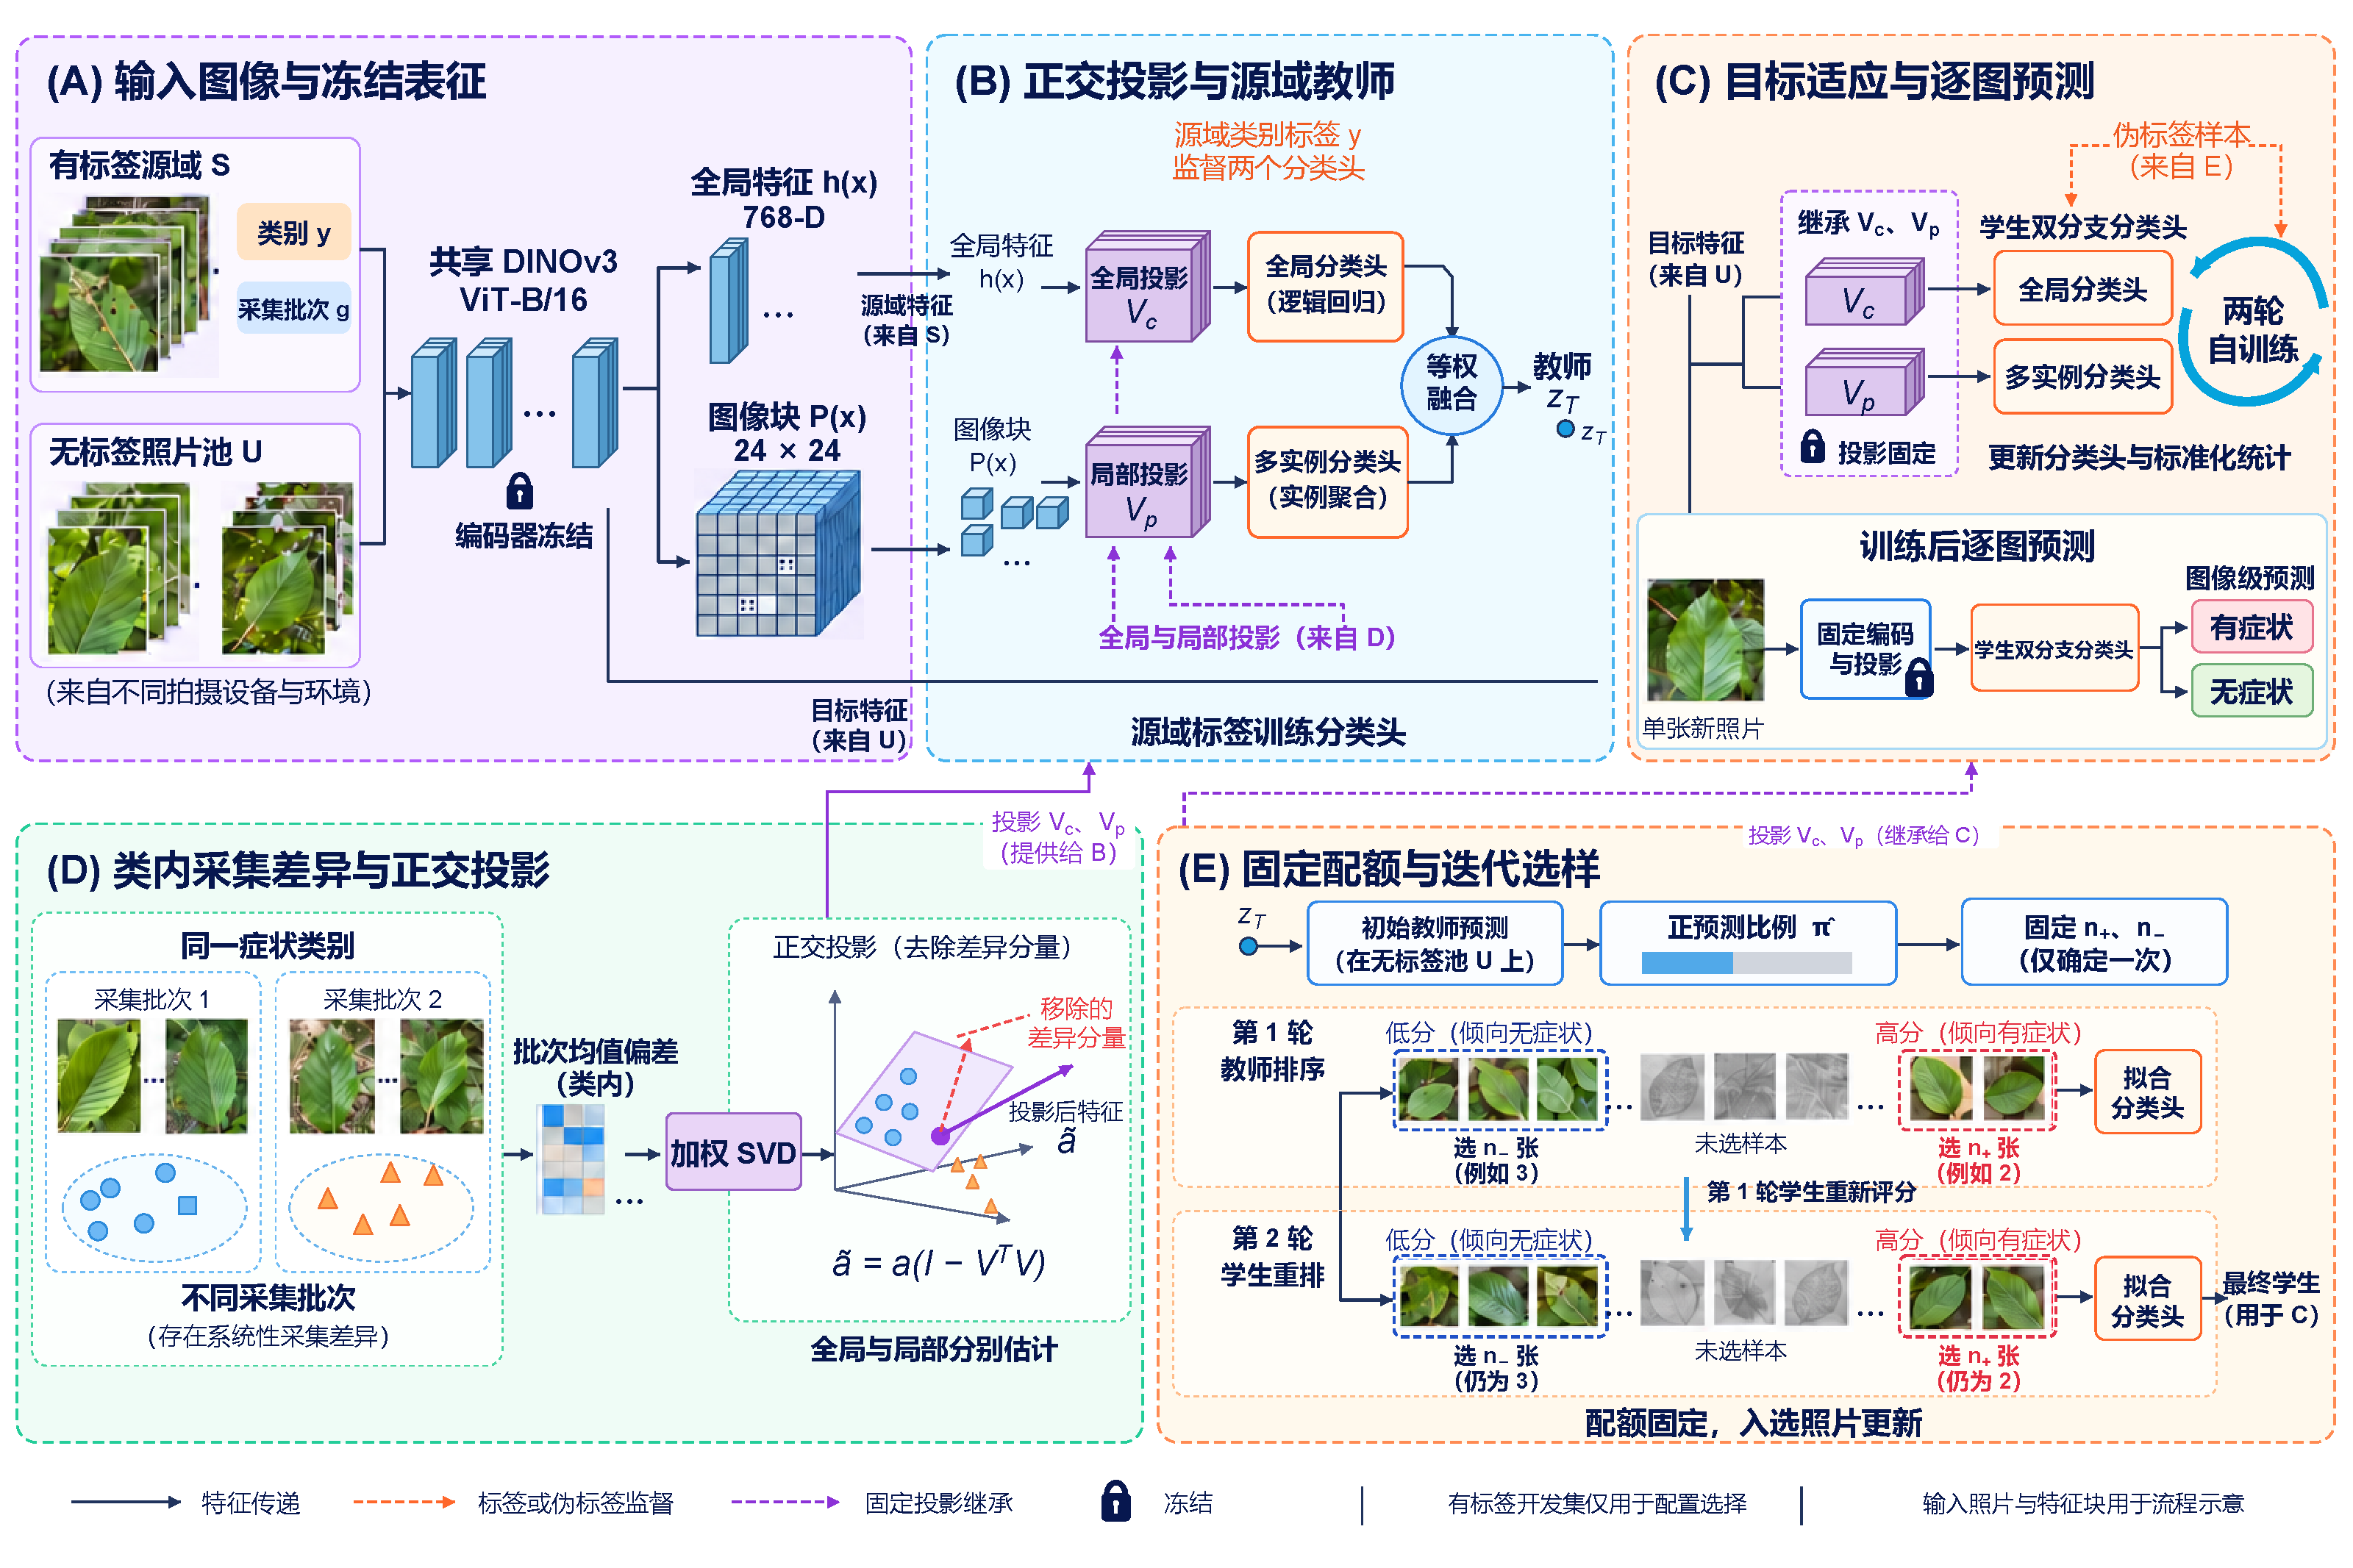
\includegraphics[width=\linewidth,height=.80\textheight,keepaspectratio]{STAND_framework_zh.pdf}
\caption{STAND 的训练与预测框架。（A）共享的冻结 DINOv3 提取全局与图像块特征。（B）源域教师融合正交投影后的全局和局部分类结果。（C）学生继承投影，在独立无标签照片池上更新分类头及标准化处理，训练后逐图预测。（D）同类采集批次差异用于估计投影方向。（E）初始教师确定两类配额，两轮自训练保持配额固定并更新入选照片。同名 $z_T$ 端口表示教师评分的传递。叶片缩略图根据照片样例生成，特征块和选样数量仅用于流程示意。开发集仅用于配置选择，外部测试图像不参与学生拟合或统计量估计。}
\label{fig:workflow}
\end{figure}

训练结束后，学生的分类头、投影基和标准化统计量保持固定。每张新照片独立经过编码、标准化、投影和两分支评分，融合分数用于有症状与无症状判定。预测不需要重新访问适应池或其他测试照片。本文的无标签蒸馏采用教师引导的硬伪标签自训练，监督来自选样后赋予照片的类别标签。

\subsection{冻结编码器与基于采集批次差异的正交投影}
本文采用 DINOv3 ViT-B/16 编码器\cite{simeoni2026}。RGB 图像先缩放至 $384\times384$，再按预训练配置进行像素标准化。编码器输出 $d=768$ 维全局特征 $h_i$ 和 $T=576$ 个图像块特征 $p_{it}\in\mathbb R^d$。图像块不包含模型的前缀标记。编码器在特征提取时使用推断模式，后续所有训练均在缓存特征上完成。

本文根据同一症状类别内不同采集批次的特征均值偏差估计主要变化方向，并通过正交投影去除特征在这些方向上的分量。为避免直接将正、负类别均值之差作为待移除方向，本文在每个类别内部估计采集批次偏差。对全局特征，用源域训练样本的逐维均值和标准差获得 $a_i=(h_i-\mu_S^c)/(\sigma_S^c+\epsilon_c)$，其中 $\epsilon_c=10^{-8}$。为利用采集批次信息，对类别 $c$ 的采集批次 $g$ 定义
\begin{equation}
D_{cg}=\sqrt{n_{cg}}\left(\bar a_{cg}-\bar a_c\right),\qquad n_{cg}\geq5,
\label{eq:deviation}
\end{equation}
其中 $\bar a_{cg}$ 和 $\bar a_c$ 分别为该类别在采集批次内和全部训练样本中的均值。将这些行向量堆叠为矩阵 $D$，对其进行奇异值分解，取前 $k$ 个右奇异向量构成行正交矩阵 $V_c$。投影后的特征为
\begin{equation}
\widetilde a_i=a_i(I-V_c^\top V_c).
\label{eq:projection}
\end{equation}
图像块使用所有源域训练图像块的均值与标准差（$\epsilon_p=10^{-6}$）标准化，再以每张图像的平均图像块表征代入式~\eqref{eq:deviation}，独立得到 $V_p$。两个分支不共享投影基。估计后的 $V_c$ 和 $V_p$ 分别用于教师的全局与图像块特征变换，并由学生在两轮训练中保持不变。

这一投影旨在压低与同类采集批次差异相关的主方向，而不是保证获得纯粹的非病害子空间。同类样本的症状程度也可能随采集批次变化，因此被移除方向可能包含有用信息。本文将 $k=0$ 作为重要对照，并在结果中单独量化投影的有限作用。

\subsection{全局—局部教师}
同一张照片的整图表征与图像块表征提供不同尺度的分类信息。本文分别对投影后的两种表征学习分类头，再融合为教师，为目标池选样提供统一分数。全局分支采用带 $L_2$ 正则的逻辑回归，输出
\begin{equation}
z_c(x)=w_c^\top\widetilde a(x)+b_c.
\end{equation}
训练采用类别平衡权重，正则参数 $C=0.1$。局部分支对每个标准化并投影的图像块共享同一线性打分器，$s_t(x)=w_p^\top\widetilde p_t(x)+b_p$，通过对数平均指数聚合得到图像分数
\begin{equation}
z_p(x)=\frac{1}{\tau}\log\left[\frac{1}{T}\sum_{t=1}^{T}\exp\bigl(\tau s_t(x)\bigr)\right],\qquad \tau=1.
\label{eq:mil}
\end{equation}
该聚合在整图标签下学习局部响应，不预先指定条带位置。局部分支采用加权二元交叉熵损失
\begin{equation}
\mathcal L_p=-\frac{1}{n}\sum_i\left[\alpha y_i\log\sigma(z_p(x_i))+(1-y_i)\log(1-\sigma(z_p(x_i)))\right],
\end{equation}
其中 $\alpha=n_-/n_+$，$\sigma$ 为 sigmoid 函数。教师以等权平均融合两个 logit，
\begin{equation}
z_T(x)=\tfrac12 z_c(x)+\tfrac12 z_p(x).
\label{eq:teacher}
\end{equation}
这避免在有限开发样本上额外拟合融合网络。局部得分图仅用于定性观察，本文不将其视为经过验证的病灶标注。

\subsection{按教师预测比例选样与学生训练}
学生训练需要确定两类各选多少张照片，以及每轮具体选择哪些照片。STAND 分别处理这两个问题。若始终从分数两端选取相同数量的照片，在一侧可靠候选较少时，可能纳入预测可靠性较低的样本。本文先以初始教师在 $\mathcal U$ 上的正预测比例确定两类数量的分配比例
\begin{equation}
\widehat\pi=\operatorname{clip}\left(\frac{1}{M}\sum_{j=1}^{M}\mathbf1[z_T(u_j)>0],\,0.05,\,0.95\right).
\end{equation}
$\widehat\pi$ 用于确定两类伪标签的数量，不代表经校准的患病率估计。令 $\rho=0.6$，正、负选样数量分别为
\begin{equation}
n_+=\max\{10,\lfloor\rho\widehat\pi M\rfloor\},\qquad
n_-=\max\{10,\lfloor\rho(1-\widehat\pi)M\rfloor\}.
\label{eq:quota}
\end{equation}
由初始教师确定的 $\widehat\pi$、$n_+$ 和 $n_-$ 在两轮中保持不变。每轮更新的是照片排序及据此构成的训练子集。在第 $r$ 轮，按照当前模型分数选取最高的 $n_+$ 张和最低的 $n_-$ 张，分别赋标签 1 和 0，构成 $\mathcal Q_r$。第一轮按教师分数选择照片，第二轮按第一轮学生对整个 $\mathcal U$ 的评分重新选择。两类数量因而不随学生的正预测比例逐轮重估，入选照片则可以随分类器更新而变化。现有实验的最小池规模为 100，选样两端无重叠，本文不对更小照片池作性能主张。

每轮学生继承源域估计的 $V_c$ 与 $V_p$，在 $\mathcal Q_r$ 的硬伪标签监督下重新拟合全局与局部分类头，默认不混入源域有标签样本。正交投影保持固定，分类权重与标准化处理根据目标照片确定，将源域的特征约束用于目标照片上的分类器学习。全局头在完整 $\mathcal U$ 的均值与标准差下拟合 $\mathcal Q_r$。局部分支先以 $\mathcal Q_r$ 中图像块的统计量训练线性打分器，再将评分时的标准化统计量替换为完整 $\mathcal U$ 的统计量，替换后不重新优化该打分器。局部分支在训练和评分时使用不同统计量，因此其性能变化同时包含分类权重和标准化处理的影响。两轮后仍按式~\eqref{eq:teacher} 融合，得到最终学生。

\subsection{训练设置与决策阈值}
源域投影维数的候选集合为 $\{0,2,4,8,12,16\}$。本文通过内部采集批次分组交叉验证选择维数，以汇总的折外 AUC 为依据。若 AUC 保留四位小数后相同，则优先选择较小维数。用于外部实验的教师采用 $k=8$。逻辑回归最多迭代 5,000 次。图像块分类头由零初始化，使用 AdamW 优化 400 步，学习率 $3\times10^{-3}$，权重衰减 $10^{-2}$，每步有放回抽取 128 张图像。主配置训练两轮学生，并另报告种子、轮数和配额系数的敏感性。

默认决策使用 $z>0$，即 sigmoid 概率阈值 0.5。为分析排序与阈值失配，另在待测批次分数上拟合双成分一维高斯混合分布，采用 200 次 EM 迭代，并在两个均值之间的 2,001 个网格点中寻找加权密度最接近的位置作为阈值。此步骤不读取标签，但读取待测批次，因此属于转导阈值调整，只在注明的诊断结果中使用，不并入外部主指标。双峰或两类均存在的条件未必成立，故该阈值规则没有一般性的可靠性保证。

\section{实验设计}
\label{sec:design}
\subsection{数据来源、标签与隔离单位}
有标签源域采用 Waldo 等公开的叶片照片，采集于 2025 年美国马里兰州\cite{waldo2026}，共包含实际可获取的 1,934 张图像，其中有症状和无症状照片分别为 787 张与 1,147 张。本文按设备和拍摄时间对照片排序，将相邻间隔不超过 300 秒的连续序列定义为一次采集批次。按此规则得到覆盖 6 个拍摄日的 23 个采集批次。以 10 秒为间隔时，照片可划分为 717 组连拍序列。采集批次刻画采集相关性，树木和叶片身份不在这一分组定义内。这一组织方式为教师训练和跨采集条件评价提供了明确的数据基础。

外部数据取自具有开放许可的 iNaturalist 照片。初始 2,999 张图像经统一内容筛选后得到 2,383 张叶片照片，覆盖 1,436 名拍摄者。筛选时使用 SigLIP~2\cite{tschannen2025} 比较叶片、树干、整树、果实及其他内容提示，仅保留叶片提示得分最高的图像。两类来源采用相同的筛选规则。每个观察记录保留一张照片，每名拍摄者每天至多保留一个观察记录。采集月份限定为 5--9 月。这一筛选流程保留叶片照片，并减少重复观察对评价的影响。症状标签按下述独立规则定义。

外部正类采用病害分类单元对应的研究级观察记录。负类采用美洲山毛榉研究级观察记录，并根据采集时设定的未报告 BLD 地域规则进行筛选。所选地域包括 Georgia、Alabama、South Carolina、Mississippi、Louisiana、Arkansas、Texas、Florida 和 Missouri。两类标签由平台鉴定和地域先验构成，属于弱标签。本文的外部指标均按这一标签定义解释。按拍摄者划分得到 527 张开发图像和 1,856 张测试图像。另设来自 2,155 名拍摄者的 2,976 张适应照片，与开发及测试拍摄者均不重合，其中病害分类单元和山毛榉分类单元来源分别为 1,381 张和 1,595 张。来源信息用于来源比例变化实验，学生训练使用教师伪标签。该划分使无标签适应的收益在新的拍摄者照片上接受检验。

\begin{table}[htbp]
\centering\small
\caption{数据划分与用途。外部正、负类按平台及地域弱标签规则定义。适应池仅用于伪标签训练。破折号表示相应训练真值或拍摄者标识未提供。}
\label{tab:data}
\begin{adjustbox}{max width=\linewidth}
\begin{tabular}{lrrrrl}
\toprule
数据 & 图像数 & 正类 & 负类 & 拍摄者数 & 用途\\
\midrule
源域 $\mathcal S$ & 1,934 & 787 & 1,147 & --- & 教师训练与采集批次评估\\
开发集 $\mathcal V$ & 527 & 294 & 233 & 343 & 配置选择\\
测试集 $\mathcal T$ & 1,856 & 1,019 & 837 & 1,093 & 外部评估\\
适应池 $\mathcal U$ & 2,976 & --- & --- & 2,155 & 伪标签学生训练\\
\bottomrule
\end{tabular}
\end{adjustbox}
\end{table}

独立目标池上的适应效果需要在未参与训练的拍摄者照片上检验。若学生直接拟合待测照片，评价会同时包含对当前批次的适配，难以判断学到的规则能否用于后续图像。本文因此将教师训练、学生适应、配置选择和外部测试的数据分别组织，具体规模见表~\ref{tab:data}。适应池与测试集的拍摄者互不重合，学生必须把一组公众照片上学得的分类规则用于新的采集者。训练完成后保持模型固定并逐图推断，使外部评价对应公众照片陆续到达时的使用方式。

公众照片中的症状线索不总以相同尺度出现在图像中。近景叶片可能占据大部分画面，多叶片场景中的同类线索则只覆盖少数区域，同时伴随背景和取景变化。源域与公众照片的样例呈现了这些差异（图~\ref{fig:examples}）。整图特征有助于保留叶片及其上下文，局部聚合则使较小的高响应区域仍能参与判断。尺度差异解释了结合两类信息的需要，采集来源的变化则说明提取特征之后还需要适应目标照片的分类规则。

\begin{figure}[htbp]
\centering
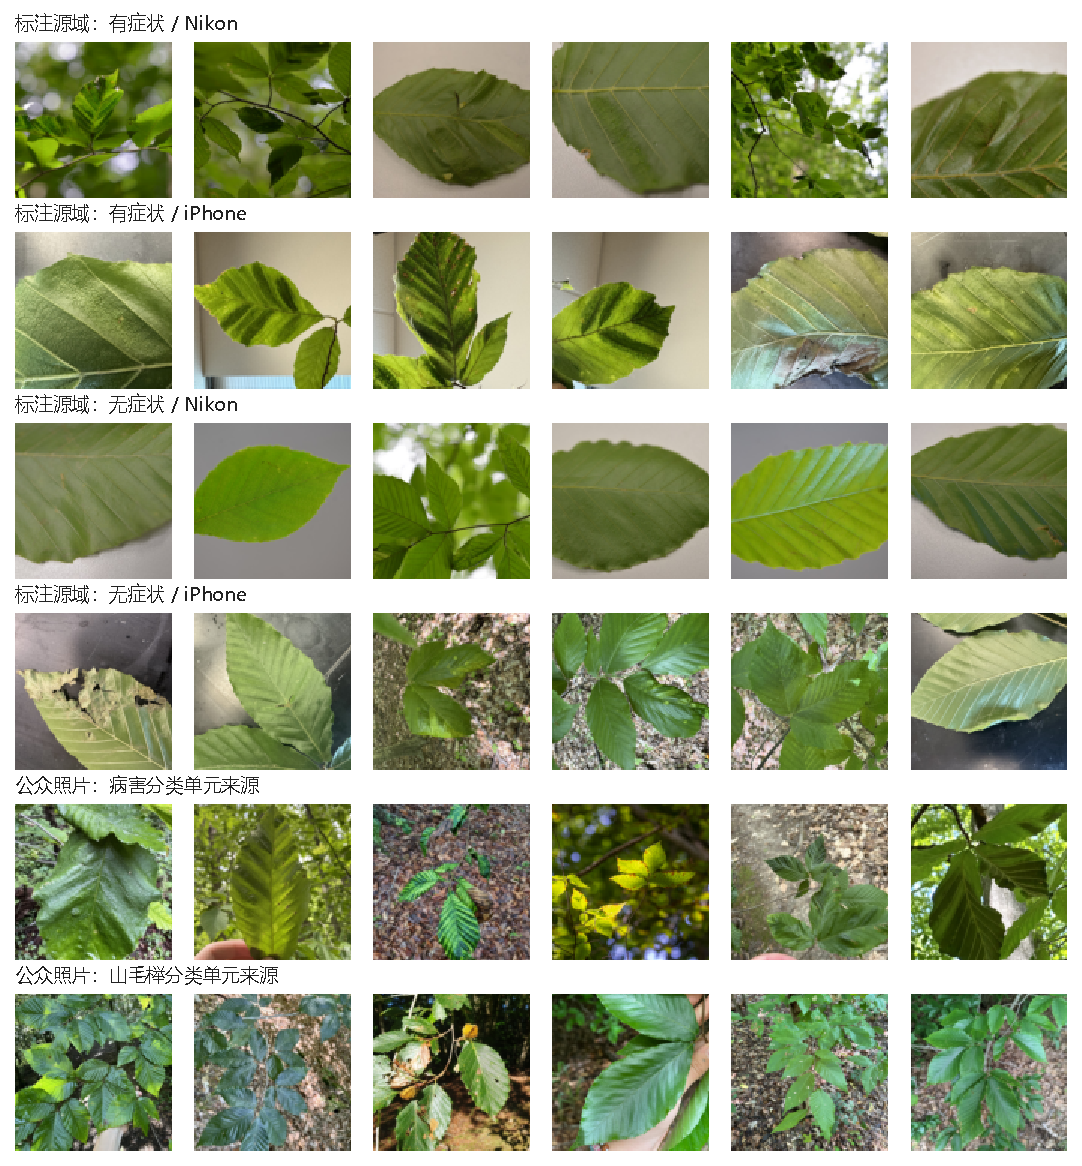
\includegraphics[width=.82\linewidth,height=.74\textheight,keepaspectratio]{fig01_examples.pdf}
\caption{源域与公众照片示例。前四行为源域类别与设备组合，后两行为公众平台病害分类单元和山毛榉分类单元来源。公众照片标签按平台与地域规则定义，负类采用采集时设定的地域筛选。}
\label{fig:examples}
\end{figure}


\subsection{比较方法与评估协议}
\label{sec:comparison}
对照系统包括已有公开 EfficientNetV2-S 检查点\cite{waldo2026}，以及在源域微调的 EfficientNetV2-S\cite{tan2021}、Inception-v3\cite{szegedy2016}、MobileNetV3-Large\cite{howard2019} 和 ResNet-50\cite{he2016}。四种 CNN 均从 ImageNet 权重开始训练，前三轮保持编码器冻结。随后，编码器与分类头的学习率分别设为 $10^{-4}$ 和 $10^{-3}$。批量大小为 16，最多训练 100 轮。验证损失连续 5 轮不改善时停止训练，并恢复验证损失最低时的权重。随机裁剪、翻转、仿射变换、灰度化和颜色扰动用于训练增强。外部对照采用原论文的模型名称，微调作为训练设置在表注中统一交代。公开检查点引用 Waldo 等的 BLD 应用论文。本文内部配置包括冻结全局分类（L1）、全局分类与正交投影（L2）以及 STAND 教师（L3），分别对应教师构建的三个阶段。L1--L3 是本文的实验配置编号，均使用 DINOv3 编码器\cite{simeoni2026}。组件分析表将这些配置与完整 STAND 进行比较。


近期表征基线采用 DINOv2-B/14\cite{oquab2024} 和 SigLIP~2-B/16\cite{tschannen2025}，分别代表自监督视觉表征与视觉语言预训练表征。两者均冻结编码器，使用缓存的整图特征训练类别平衡的逻辑回归，不加入正交投影、局部分支或目标池适应。输入边长分别为 392 和 224。特征逐维标准化的统计量仅由源域拟合样本计算。正则参数 $C$ 的候选集合为 $\{0.001,0.01,0.1,1,10\}$，选择依据为源域五折采集批次分组验证的汇总折外 AUC。若 AUC 保留四位小数后相同，则优先选择较小 $C$。DINOv2 和 SigLIP~2 最终分别选择 10 和 1。选定后在全部 1,934 张源域图像上拟合分类头，以零分数阈值评价同一外部测试集。两项基线均按预定候选范围报告，外部标签不参与参数选择。上述结果来自本研究补充的源域线性探测实验。附录表~\ref{tab:backbone} 中的 DINOv2 采用正交投影和不同的分类头配置，用于评价投影后的表征表现。

内部评估采用以完整采集批次为单位的五折分层分组交叉验证，每次留出一折测试。CNN 使用下一折验证，在另外三折更新参数。冻结分类头使用全部非测试折拟合，并在这一范围内通过嵌套采集批次验证选择投影维数。两类方法的监督拟合预算据此分别报告。另以“拍摄日 $\times$ 设备”形成 7 个组进行留一检验。采集批次与日—设备两级分组分别考察局部连续采集和更大采集单元的变化，为全局—局部教师的跨条件表现提供互补证据。

外部评价统一使用表~\ref{tab:data} 中的公众照片测试集。冻结教师在全部 1,934 张源域图像上拟合，四种微调 CNN 在按 70/15/15 划分的源域训练部分更新参数、使用验证部分早停，并报告三个种子的均值。主表比较外部对照与完整 STAND 的系统表现，各方法的预训练规模、模型结构和源域拟合预算有所不同。组件分析表中的内部配置共享编码器，用于分析固定表征条件下的增益来源。这两个层次分别回答 STAND 的整体识别表现和增益来源，使性能比较与创新论证相互衔接。

评价指标包括准确率、精确率、召回率、F1 和 ROC-AUC。其中，有症状照片作为正类。表格和结果分析中的 AUC 乘以 100。准确率及 F1 描述整体决策，召回率和精确率分别反映遗漏与报阳质量，AUC 则刻画跨阈值排序。外部结果采用 1,000 次拍摄者聚类 bootstrap。每次有放回地抽取拍摄者，并保留其对应的全部照片。采样区间取第 2.5 和第 97.5 百分位。结果按描述性比较报告，不作配对显著性声明。采集批次 AUC 先逐折计算再平均，准确率合并各折预测计算，使排序与决策的评价各自对应明确的统计口径。

\subsection{模型选择与测试暴露}
配置选择使用有标签开发集，比较伪标签规则、训练轮数、投影、源域样本混入和标准化处理。本文所称的“无标签”仅指学生拟合阶段使用的适应池。研究记录显示，开发期间曾查看早期较小照片池上 15 个配置的外部测试表现。现有记录未将这些成绩列为最终配置选择依据。按教师预测比例选样的规则也受到照片池组成分析的启发。外部测试按拍摄者隔离开展，来源比例变化实验用于探索选样规则的适用条件。由于开发期间曾查看部分测试结果，该测试集不属于全过程未接触的确认性留出集。将开发选择与学生训练的数据角色明确区分，有助于准确评价现有证据所支持的跨来源适应能力。


\section{实验结果}
\label{sec:results}
本文以完整 STAND 为参照，依次考察共同外部测试上的整体性能、组件递进与学生消融、目标池条件变化，以及输出分数和具体案例。组件实验保持测试照片一致，并说明每种配置相对完整方法改变的环节。源域教师的逐折结果、表征和聚合选择集中于附录~\ref{app:teacher}，用于解释教师初始化。
\subsection{公众照片上的跨来源识别}
首先考察在保持视觉表征固定的条件下，公众照片能否为分类器提供有效的适应信息。实验设置包括源域分类器、全局—局部教师和目标池学生，并在同一外部测试集上评价。L3 与 STAND 采用相同的冻结编码器和分类头结构，学生阶段仅更新分类权重及特征统计量，因此二者的差异可用于分析目标池学习的作用。主比较同时纳入公开模型和微调 CNN，以评价完整系统的外部表现，结果汇总于表~\ref{tab:external}。主表中的方法名称对应所引用的架构或公开检查点，完整 STAND 的内部配置另见表~\ref{tab:ladder}。共享编码器的教师—学生对照用于解释适应收益，外部模型对照用于描述不同系统在当前公众照片上的识别表现。

\begin{table}[htbp]
\centering\small
\caption{公众照片测试集上的主性能对比，包含 1,856 张图像及 1,093 名拍摄者。指标均由本文测量并以百分数表示，$\uparrow$ 表示越高越好。前三种 CNN 报告源域微调三个种子的均值。DINOv2 与 SigLIP~2 使用冻结编码器和源域线性分类头，其余均为单模型。EfficientNetV2-S 使用 Waldo 等的公开检查点，其年份为 BLD 应用论文年。其他对照标注模型论文年份，SigLIP~2 为 2025 年预印本。训练与预训练预算见第~\ref{sec:comparison} 节。各列最高值加粗，显示精度下并列最高均加粗。}
\label{tab:external}
\begin{adjustbox}{max width=\linewidth}
\begin{tabular}{lrrrrrr}
\toprule
方法与引用 & 年份 & 准确率$\uparrow$ & 精确率$\uparrow$ & 召回率$\uparrow$ & F1$\uparrow$ & AUC$\uparrow$\\
\midrule
Inception-v3\cite{szegedy2016} & 2016 & 71.17 & 87.74 & 57.34 & 67.00 & 85.24\\
MobileNetV3-Large\cite{howard2019} & 2019 & 69.31 & 89.80 & 51.13 & 63.73 & 84.46\\
ResNet-50\cite{he2016} & 2016 & 71.26 & 90.82 & 53.06 & 66.82 & 85.10\\
DINOv2-B/14\cite{oquab2024} & 2024 & 77.59 & \textbf{99.18} & 59.67 & 74.51 & 95.71\\
SigLIP~2-B/16\cite{tschannen2025} & 2025 & 71.34 & 89.59 & 54.07 & 67.44 & 85.17\\
EfficientNetV2-S\cite{waldo2026} & 2026 & 81.30 & 81.00 & 86.16 & 83.50 & 89.64\\
\midrule
\textbf{STAND（本文）} & 2026 & \textbf{91.38} & 93.87 & \textbf{90.19} & \textbf{91.99} & \textbf{97.25}\\
\bottomrule
\end{tabular}
\end{adjustbox}
\end{table}


症状筛查需要同时考虑检出数量和报阳质量，较高的精确率需要结合召回率解释。DINOv2 线性探测取得 95.71 的 AUC，说明冻结表征已能提供较强的跨来源排序信息。其默认阈值下的精确率为 99.18\%，召回率为 59.67\%。这一结果表明，较少的误报同时伴随较多遗漏。SigLIP~2 线性探测的召回率为 54.07\%，也体现出源域决策用于公众照片时的检出不足。STAND 在 93.87\% 精确率下达到 90.19\% 召回率，并取得表中最高的准确率、F1 和 AUC（表~\ref{tab:external}）。该结果支持将可迁移表征与目标来源的决策学习结合，而不只依赖源域分类头直接迁移。不同编码器之间的比较评价完整系统表现。目标池适应的具体作用由共享 DINOv3 编码器的教师与学生对照检验。

上述决策改善还需要与阈值变化区分。准确率会随阈值位置改变，而 AUC 取决于正、负样本的相对排序，因而能够检验学生是否学到了不同的判别关系。ROC 对照中，学生的 AUC 从教师的 95.09 提高到 97.25（图~\ref{fig:roc}）。移动固定教师分数上的阈值不会产生这一变化，说明适应收益包含样本区分能力的改善。学生在目标特征上重新拟合分类头并更新统计量，使同一编码器输出的特征形成更适合公众照片的分数。该结果为固定表征上的分类器学习提供了直接支持。

\begin{figure}[htbp]
\centering
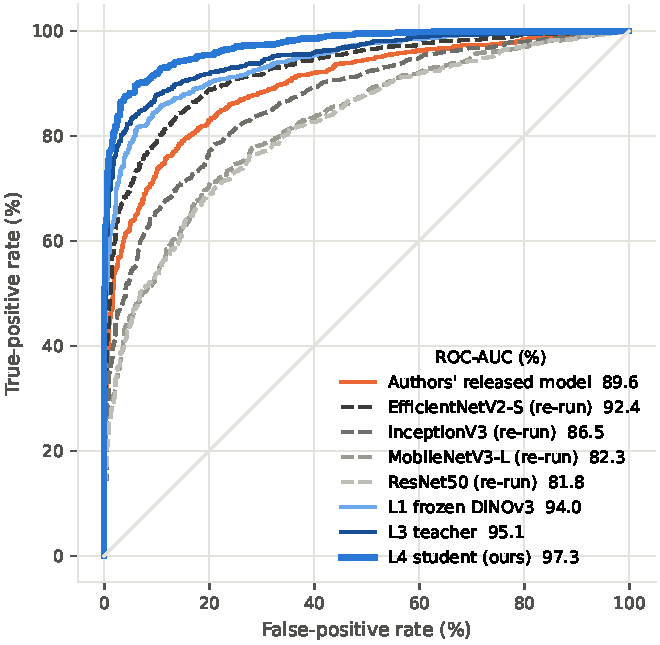
\includegraphics[width=.68\linewidth,height=.74\textheight,keepaspectratio]{fig08_roc_external.pdf}
\caption{公众照片外部测试的 ROC 曲线。图中 L4 student 指 STAND。CNN 曲线使用种子 0 的单个模型，因此图例 AUC 与主表三个种子的均值可能不同。公开模型和 STAND 对应主表的单模型。L1 与 L3 对应表~\ref{tab:ladder} 的内部配置。}
\label{fig:roc}
\end{figure}

同一拍摄者提交的照片可能共享设备、取景和场景，逐张图像重采样难以保留这种关联。为考察当前结果对拍摄者构成变化的敏感性，我们以拍摄者为单位进行整体重采样，并计算固定模型的性能区间。STAND 的准确率区间为 90.07\%--92.78\%，AUC 区间为 96.59--97.87，具体分布见图~\ref{fig:extbars}。排序与决策在这一采样口径下均保持较好表现，为主表的点估计补充了不确定性信息，也支持独立目标池训练的分类器用于新的拍摄者照片。该区间描述当前测试人群的采样变化，不包含模型选择偏差。

\begin{figure}[htbp]
\centering
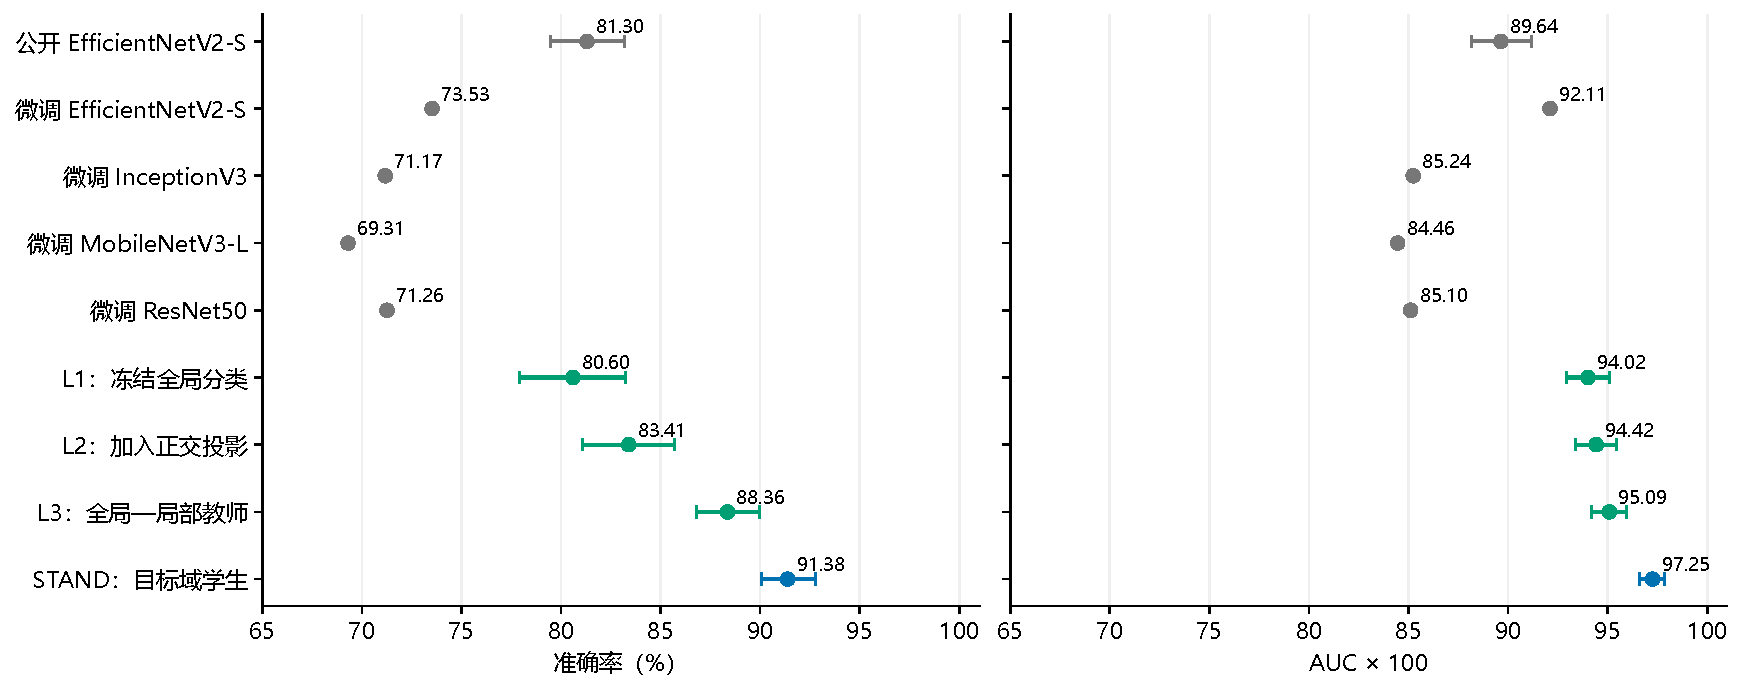
\includegraphics[width=1.0\linewidth,height=.74\textheight,keepaspectratio]{fig09_external_bars.pdf}
\caption{STAND 与对照方法的外部性能及不确定性。带误差线的点表示单模型结果。误差线为拍摄者聚类 bootstrap 95\% 区间。四种 CNN 基线用无区间的点标示三个种子的均值。L1--L3 为表~\ref{tab:ladder} 的本文内部配置。}
\label{fig:extbars}
\end{figure}


\subsection{从源域分类器到完整 STAND 的组件递进}
为解释完整 STAND 的性能来源，我们在同一公众照片测试集上比较 L1、L2、L3 与完整方法。L1 只使用冻结全局表征，L2 加入正交投影，L3 增加局部分支，STAND 再利用独立目标池学习学生分类器。各配置共享编码器，因此能够在表征保持不变的条件下，分别观察采集批次处理、局部信息和目标池学习如何影响最终决策。表~\ref{tab:ladder} 汇总这一递进过程，并同时报告精确率与召回率，以区分误报控制和症状检出的变化。

\begin{table}[htbp]
\centering\small
\caption{本文内部配置与完整 STAND 的组件递进结果（\%）。各配置共享 DINOv3 编码器及同一外部测试集。L1 仅采用全局分类头，L2 在其基础上加入正交投影，L3 再加入局部分支形成教师，完整 STAND 执行目标池学生适应。L1--L3 是本文的实验配置编号，不对应独立发表的方法。各性能列最高值加粗。}
\label{tab:ladder}
\begin{adjustbox}{max width=\linewidth}
\begin{tabular}{lrrrrr}
\toprule
本文配置 & 准确率$\uparrow$ & 精确率$\uparrow$ & 召回率$\uparrow$ & F1$\uparrow$ & AUC$\uparrow$\\
\midrule
冻结全局分类（L1） & 80.60 & 97.41 & 66.44 & 79.00 & 94.02\\
全局分类与正交投影（L2） & 83.41 & \textbf{97.98} & 71.25 & 82.50 & 94.42\\
STAND 教师（L3） & 88.36 & 93.98 & 84.20 & 88.82 & 95.09\\
STAND（完整方法） & \textbf{91.38} & 93.87 & \textbf{90.19} & \textbf{91.99} & \textbf{97.25}\\
\bottomrule
\end{tabular}
\end{adjustbox}
\end{table}


整图表征把图像压缩为一个向量，局部分支则保留各区域对分类分数的贡献。加入局部头后，部分照片能够越过决策阈值，而不必显著重排所有样本。L2 到 L3 的召回率由 71.25\% 提高到 84.20\%，准确率的改善也大于 AUC 的变化，说明局部信息的补充主要体现为正类检出增加（表~\ref{tab:ladder}）。学生适应随后继续改善排序和默认阈值准确率，支持先结合整图与区域信息建立教师，再利用公众照片学习目标分类规则的设计。

\subsection{以完整 STAND 为参照的消融分析}
组件对照需要明确每项实验改变的环节。我们以完整 STAND 为参照，分别移除学生局部分支、关闭学生正交投影、改用仅含全局头的初始教师，以及在学生拟合中加入源域标签。未适应的 L3 教师作为参照，用于评价目标池学生学习的整体作用。各项对照列于表~\ref{tab:ablation}，选样比例、训练轮数、标准化与随机种子按完整实验组列于附录~\ref{app:student_settings}。

\begin{table}[htbp]
\centering\small
\caption{完整 STAND 的组件与训练策略对照（\%）。各行相对完整方法改变注明环节，其他设置保持一致。L3 教师为适应前参照。两类等量选样与 STAND 主配置的伪标签数量分别为 1,784 和 1,785。选样比例、训练轮数、标准化及随机种子结果见补充表~\ref{tab:student_settings}。开发与测试数据的使用情况见第~\ref{sec:comparison} 节。各性能列最高值加粗，伪标签数量仅描述训练规模。}
\label{tab:ablation}
\begin{adjustbox}{max width=\linewidth}
\begin{tabular}{lrrrrrr}
\toprule
配置 & 伪标签数 & 开发 AUC & 开发准确率 & 测试 AUC & 测试准确率 & \makecell{测试调整\\阈值准确率}\\
\midrule
未执行学生适应（L3 教师） & --- & --- & --- & 95.09 & 88.36 & 88.42\\
两类等量选样（两端各 30\%） & 1784 & 97.69 & 93.55 & 97.07 & 90.57 & 90.95\\
移除学生局部分支 & 1785 & 96.97 & 90.70 & 96.02 & 87.98 & 89.33\\
移除学生正交投影 & 1785 & 97.64 & 93.36 & 97.05 & 91.06 & \textbf{91.06}\\
使用仅全局教师生成伪标签 & 1785 & 97.62 & 91.46 & 97.20 & 90.62 & 91.00\\
学生训练加入源域标签 & 1785 & 96.92 & 91.08 & 96.58 & 90.25 & 90.41\\
\textbf{STAND（完整方法）} & 1785 & \textbf{97.85} & \textbf{93.74} & \textbf{97.25} & \textbf{91.38} & \textbf{91.06}\\
\bottomrule
\end{tabular}
\end{adjustbox}
\end{table}


局部响应在适应后仍为分类提供补充。移除学生局部分支后，测试 AUC 从 97.25 降至 96.02，默认准确率从 91.38\% 降至 87.98\%。这两项指标的下降支持在学生中保留区域判别信息。关闭正交投影或采用仅全局教师时，学生仍保持较强表现，但均低于完整设置。不同幅度的变化说明，全局与局部信息的联合使用是当前组件收益的重要来源，正交投影和教师配置则影响这一收益的具体大小。

伪标签选样还决定了学生拟合时所见的类别组成。固定两端各 30\% 与按教师预测比例选样的主配置使用相近的样本数量，后者取得更好的排序与默认准确率，支持按教师估计的类别组成分配训练样本。将源域有标签样本再次混入学生训练也没有超过目标池单独拟合的完整设置，说明教师已传递的判别信息可以与面向公众照片的分类器学习配合。两类对照分别支持按教师预测比例选样和目标池拟合，其在不同照片池条件下的表现由后续敏感性实验评价。

\subsection{STAND 对照片池规模与组成变化的适应}
实际应用中可获得的无标签公众照片数量可能有限，因此有必要检查适应是否必须依赖较大的目标池。学生已经继承冻结编码器和源域教师提供的判别基础，目标照片主要用于重新拟合分类规则，这与从头学习视觉表征的数据需求不同。缩小照片池后，仅使用 100 张照片的平均 AUC 已达到 96.84，并超过未适应教师（表~\ref{tab:pool}）。该结果验证了少量无标签数据也能支持当前任务的分类器适应。随着照片池扩大，平均收益没有单调增加，说明数量之外还需要考虑所抽到的来源及可用伪标签，组成实验据此检查另一项数据条件。

\begin{table}[htbp]
\centering\small
\caption{STAND 及固定配额变体对无标签池数量与组成的敏感性（\%）。范围为两次运行的最小值至最大值，完整池为单次主配置。组成按病害分类单元检索来源计数。每个实验区的平均性能列最高值加粗。}
\label{tab:pool}
\begin{adjustbox}{max width=\linewidth}
\begin{tabular}{lrrrrr}
\toprule
照片池条件 & 次数 & STAND AUC & 运行范围 & STAND 准确率 & \makecell{固定配额变体\\AUC}\\
\midrule
\multicolumn{6}{l}{\textit{数量实验}}\\
\addlinespace[2pt]
100 张 & 2 & 96.84 & 96.18--97.51 & 90.17 & ---\\
200 张 & 2 & 96.34 & 96.34--96.35 & 88.50 & ---\\
400 张 & 2 & 96.97 & 96.54--97.40 & 90.38 & ---\\
800 张 & 2 & 97.08 & 96.63--97.53 & 90.76 & ---\\
1,600 张 & 2 & 97.04 & 97.00--97.08 & 90.73 & ---\\
2,976 张（完整池） & 1 & \textbf{97.25} & --- & \textbf{91.38} & \textbf{97.07}\\
\midrule
\multicolumn{6}{l}{\textit{组成实验，每池 1,000 张，病害分类单元来源比例}}\\
\addlinespace[2pt]
5\% & 2 & 95.37 & 95.25--95.50 & 87.90 & 87.35\\
10\% & 2 & 95.82 & 95.43--96.21 & 88.44 & 89.22\\
20\% & 2 & 96.95 & 96.74--97.15 & 90.03 & 93.52\\
35\% & 2 & 96.96 & 96.72--97.20 & 90.41 & 96.53\\
50\% & 2 & \textbf{97.35} & 96.92--97.78 & \textbf{91.46} & \textbf{97.23}\\
65\% & 2 & 97.05 & 96.82--97.29 & 90.52 & 96.33\\
80\% & 2 & 95.81 & 95.59--96.03 & 88.28 & 94.56\\
90\% & 2 & 93.58 & 92.81--94.35 & 85.61 & 93.86\\
95\% & 2 & 92.15 & 91.71--92.58 & 84.05 & 93.14\\
\bottomrule
\end{tabular}
\end{adjustbox}
\end{table}


相同数量的目标照片也可能形成不同的两类候选分布。两类等量选样始终要求两端选入同样多的样本，当一侧可靠候选较少时，可能被迫纳入置信度较低的照片。按教师预测比例选样的规则则根据初始教师预测分配两端数量，允许选样随当前池变化。在接近平衡的来源条件下，两种规则表现接近。当病害来源占比降到 5\% 时，差距扩大到约 8.02 个 AUC 点（图~\ref{fig:pool}）。收益随来源偏斜加大，与两种规则在选样约束上的差异相符，验证了按池组成调整伪标签配额在该条件下的作用。

\begin{figure}[htbp]
\centering
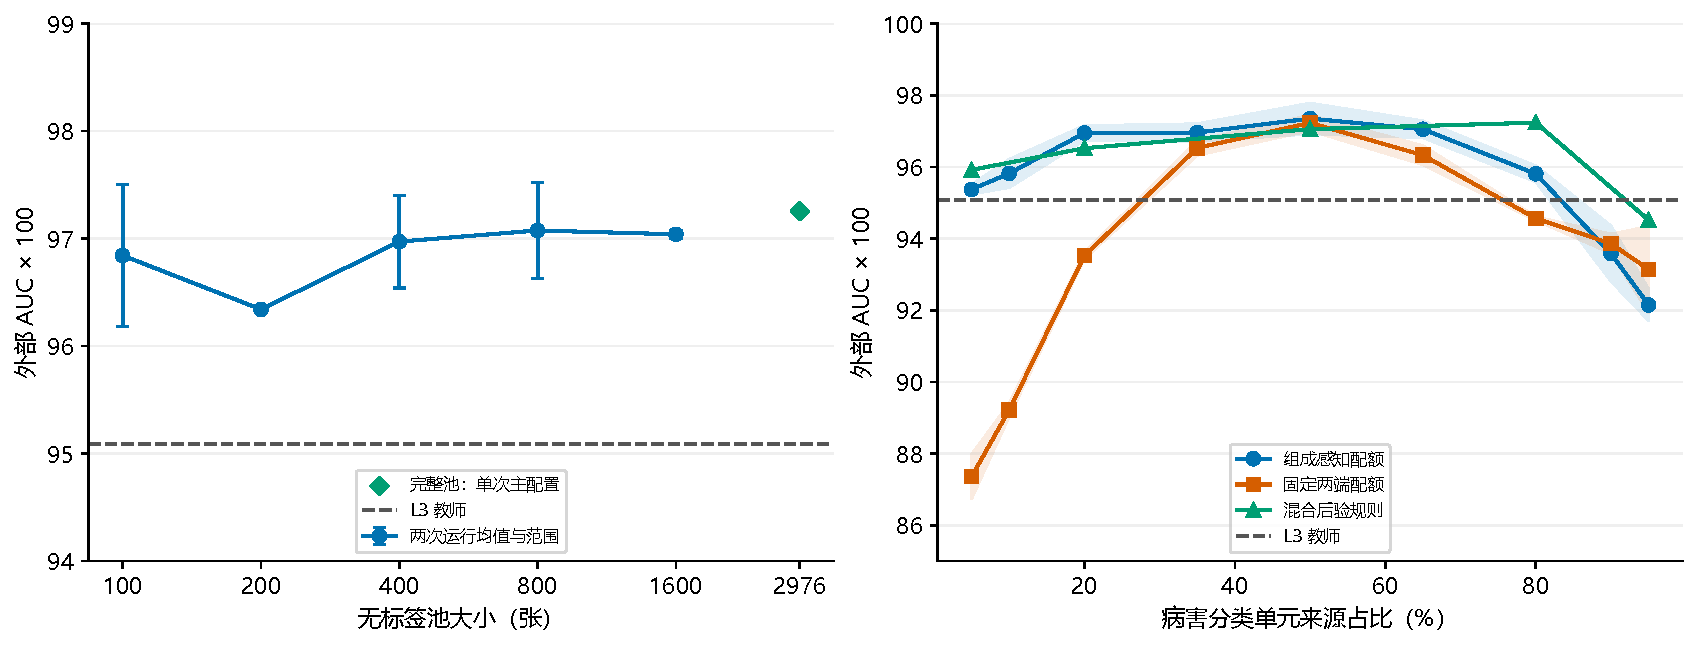
\includegraphics[width=1.0\linewidth,height=.74\textheight,keepaspectratio]{fig16_pool_sensitivity.pdf}
\caption{STAND 的无标签池规模与组成敏感性。按教师预测比例选样的曲线为 STAND，固定配额和混合后验为伪标签选择变体。左侧误差线及右侧色带为两次运行的最小值至最大值。完整池和混合后验对照为单次结果。虚线为教师 AUC，两个面板纵轴范围不同。右侧比例按照片检索来源定义。}
\label{fig:pool}
\end{figure}

当照片池进一步接近单一来源时，配额调整能够利用的信息也随之改变。在 20\%--65\% 的来源比例下，按教师预测比例选样的规则保持较稳定收益。比例达到 90\% 和 95\% 时，AUC 分别降至 93.58 和 92.15。在 95\% 条件下，固定配额与混合后验的结果也低于教师。多种选择规则的共同下降说明，调整两端数量不能补充照片池中缺失的类别与来源信息，教师组成估计的偏差还可能进入学生训练。因此，按教师预测比例选样用于改善已有候选的分配，而来源覆盖为这种选择提供必要基础。二者应在组织目标照片时共同考虑。

\subsection{分类排序、决策阈值与概率校准}
较好的样本排序只有转化为合适的类别决策，才能直接用于逐图筛查。部署时保持阈值固定尤其需要适应后的分数与目标照片分布相匹配，因此我们观察正、负类分数相对默认阈值和混合分布阈值的位置。STAND 的默认准确率与无标签调整阈值后的结果接近，且前者略高，分数分布见图~\ref{fig:scores}。这一结果说明当前目标池训练已得到可直接使用的决策位置。结合前述 AUC 提升，学生适应同时改善了排序和固定阈值下的分类表现，使后续照片可以逐图预测。

\begin{figure}[htbp]
\centering
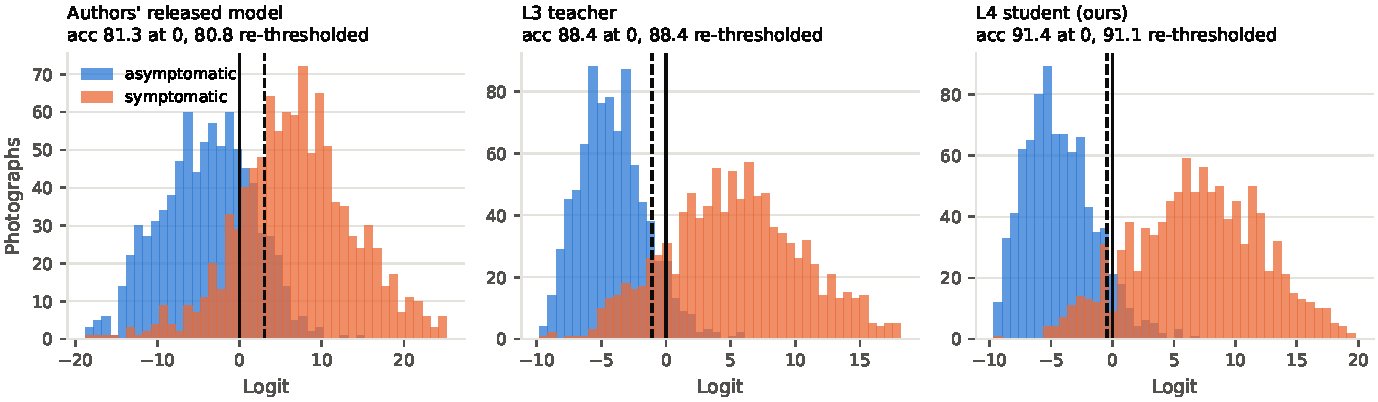
\includegraphics[width=1.0\linewidth,height=.74\textheight,keepaspectratio]{fig11_score_distributions.pdf}
\caption{STAND 与源域分类器的外部正、负类分数直方图。图中 L4 student 为完整 STAND。实线为默认 logit 阈值 0，虚线为无标签混合分布阈值。两类名称按外部弱标签定义理解。每个面板纵轴为照片数量。}
\label{fig:scores}
\end{figure}

为检查学生的优势是否仍取决于默认阈值，我们对教师和学生分别采用相同的无标签阈值调整规则。学生在默认与调整阈值两种条件下均优于教师，具体结果见表~\ref{tab:external_details}。这种一致性说明，单独修正教师的决策位置并未消除二者的差距。结合图~\ref{fig:roc} 的 AUC 变化，实验支持重新拟合分类头能够获得阈值修正之外的判别收益，验证了用目标照片学习全局与局部分类规则的作用。

\begin{table}[htbp]
\centering\small
\caption{外部测试的采样区间与阈值对照，指标按百分数表示。区间为单模型的拍摄者聚类 bootstrap 95\% 区间。四种微调 CNN 报告三个种子的指标均值。点估计的列最高值加粗。}
\label{tab:external_details}
\begin{adjustbox}{max width=\linewidth}
\begin{tabular}{lrrrrr}
\toprule
方法 & 准确率 & 准确率区间 & AUC & AUC 区间 & \makecell{调整阈值\\准确率}\\
\midrule
公开 EfficientNetV2-S\cite{tan2021,waldo2026} & 81.30 & 79.48--83.20 & 89.64 & 88.18--91.17 & 80.77\\
微调 EfficientNetV2-S\cite{tan2021} & 73.53 & --- & 92.11 & --- & 80.44\\
微调 Inception-v3\cite{szegedy2016} & 71.17 & --- & 85.24 & --- & 73.76\\
微调 MobileNetV3-Large\cite{howard2019} & 69.31 & --- & 84.46 & --- & 63.81\\
微调 ResNet-50\cite{he2016} & 71.26 & --- & 85.10 & --- & 72.97\\
L1 冻结全局分类\cite{simeoni2026} & 80.60 & 77.90--83.24 & 94.02 & 92.94--95.07 & 86.75\\
L2 加入正交投影 & 83.41 & 81.08--85.71 & 94.42 & 93.37--95.42 & 87.18\\
L3 全局—局部教师 & 88.36 & 86.79--89.96 & 95.09 & 94.18--95.96 & 88.42\\
\textbf{STAND（本文）} & \textbf{91.38} & 90.07--92.78 & \textbf{97.25} & 96.59--97.87 & \textbf{91.06}\\
\bottomrule
\end{tabular}
\end{adjustbox}
\end{table}


除了类别是否判断正确，输出概率与目标标签频率的一致性也是值得检查的性质。AUC 只评价相对排序，可靠性曲线则比较相近预测概率下实际观测到的正类比例。我们没有额外拟合概率校准器，而是直接检查教师与学生的输出，经验校准误差由约 5.6\% 降至 3.5\%（图~\ref{fig:calib}）。这一变化与准确率和 AUC 的改善同时出现，说明目标池学习既增强了类别区分，也使分数分布更接近当前弱标签频率。校准收益伴随目标样本拟合和统计处理产生，其概率含义仍限于当前标签定义。

\begin{figure}[htbp]
\centering
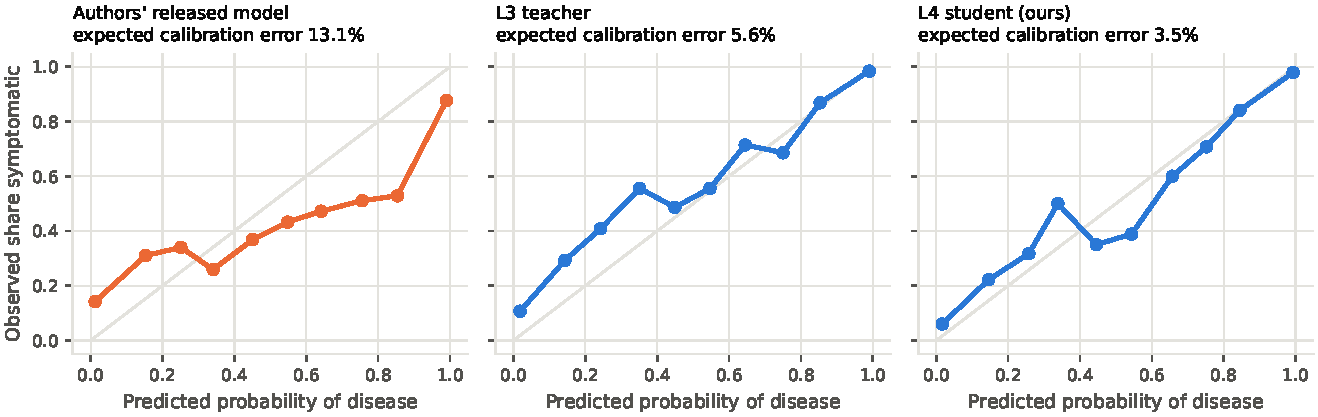
\includegraphics[width=1.0\linewidth,height=.74\textheight,keepaspectratio]{fig19_calibration.pdf}
\caption{STAND 与源域分类器的外部可靠性图。图中 L4 student 为完整 STAND。概率按 10 个等宽区间分箱，连线仅显示样本数至少 15 的箱。ECE 使用所有非空箱按样本比例加权计算。对角线为理想经验校准。}
\label{fig:calib}
\end{figure}

\subsection{分层表现、局部响应与失败案例}
总体成绩还可能受到不同年份和来源样本数量的影响，因此我们将外部结果按采集年份和地域字段展开。年度子集用于检查收益是否集中于单个时期，地域子集则分别观察正类检出与负类排除。STAND 在 2021--2026 年各年度均优于公开模型，分组表现见图~\ref{fig:strata}。这种一致性说明总体改善具有多个采集条件下的支持，而非仅由某一年贡献。正、负类采用不同来源规则，故各地域结果按其样本量作描述性解释，用于补充总体适应结论的适用范围。

\begin{figure}[htbp]
\centering
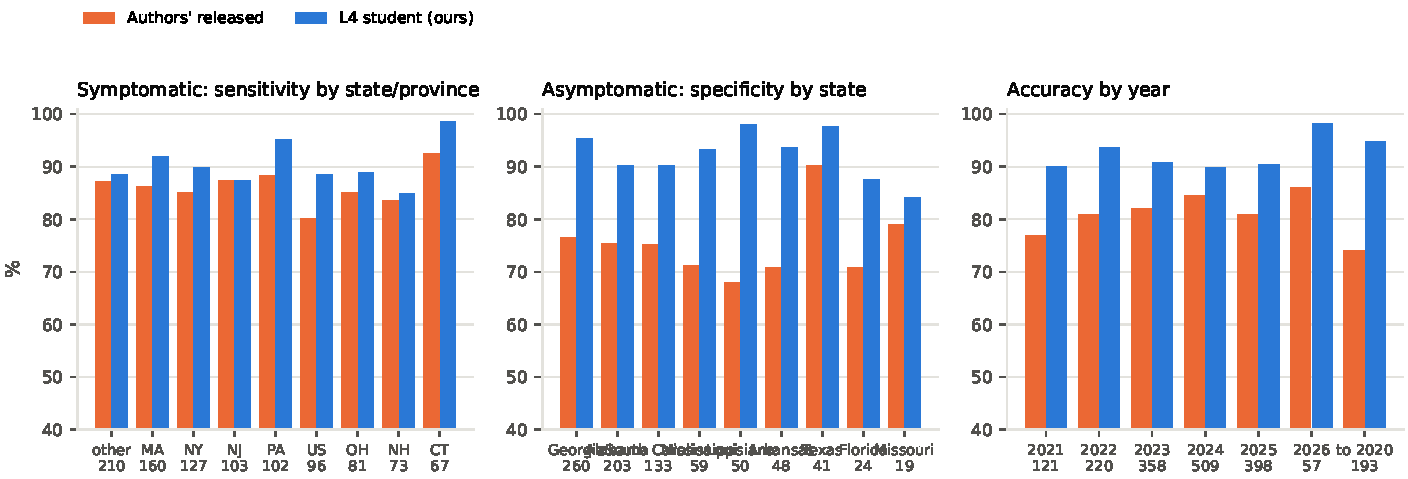
\includegraphics[width=1.0\linewidth,height=.74\textheight,keepaspectratio]{fig20_strata.pdf}
\caption{STAND 与公开模型按地域字段及年份分组的外部表现。前两图分别在正类和负类内报告灵敏度与特异度。第三图报告各年准确率。横轴第二行列出样本数。US 与 other 保留原始位置字符串的分组含义。各分组显示描述性点估计。}
\label{fig:strata}
\end{figure}

局部信息的补充作用可以结合具体照片的分类变化理解。图~\ref{fig:maps} 先标出每例的数据标签与两个模型的判断，再并列原图、公开模型的 Grad-CAM\cite{selvaraju2017} 和 STAND 图像块得分。A 组展示公开模型漏检而 STAND 检出的照片，B 组展示两者均正确的照片，C 组展示 STAND 纠正公开模型误报的照片。近景叶片和多叶片场景中均出现纠正案例，说明所选样例的收益同时涉及症状检出和负类排除。结合表~\ref{tab:ablation} 中移除局部分支后的性能变化，这些观察为全局与局部信息的互补作用提供了定性支持。STAND 热图的蓝色和橙色分别表示局部得分偏向无症状和有症状，公开模型的亮色则表示该图中较强的有症状类别响应。两种热图使用不同定义，区域响应应与最终预测一起阅读，不能由颜色直接判断病斑位置。

\begin{figure}[htbp]
\centering
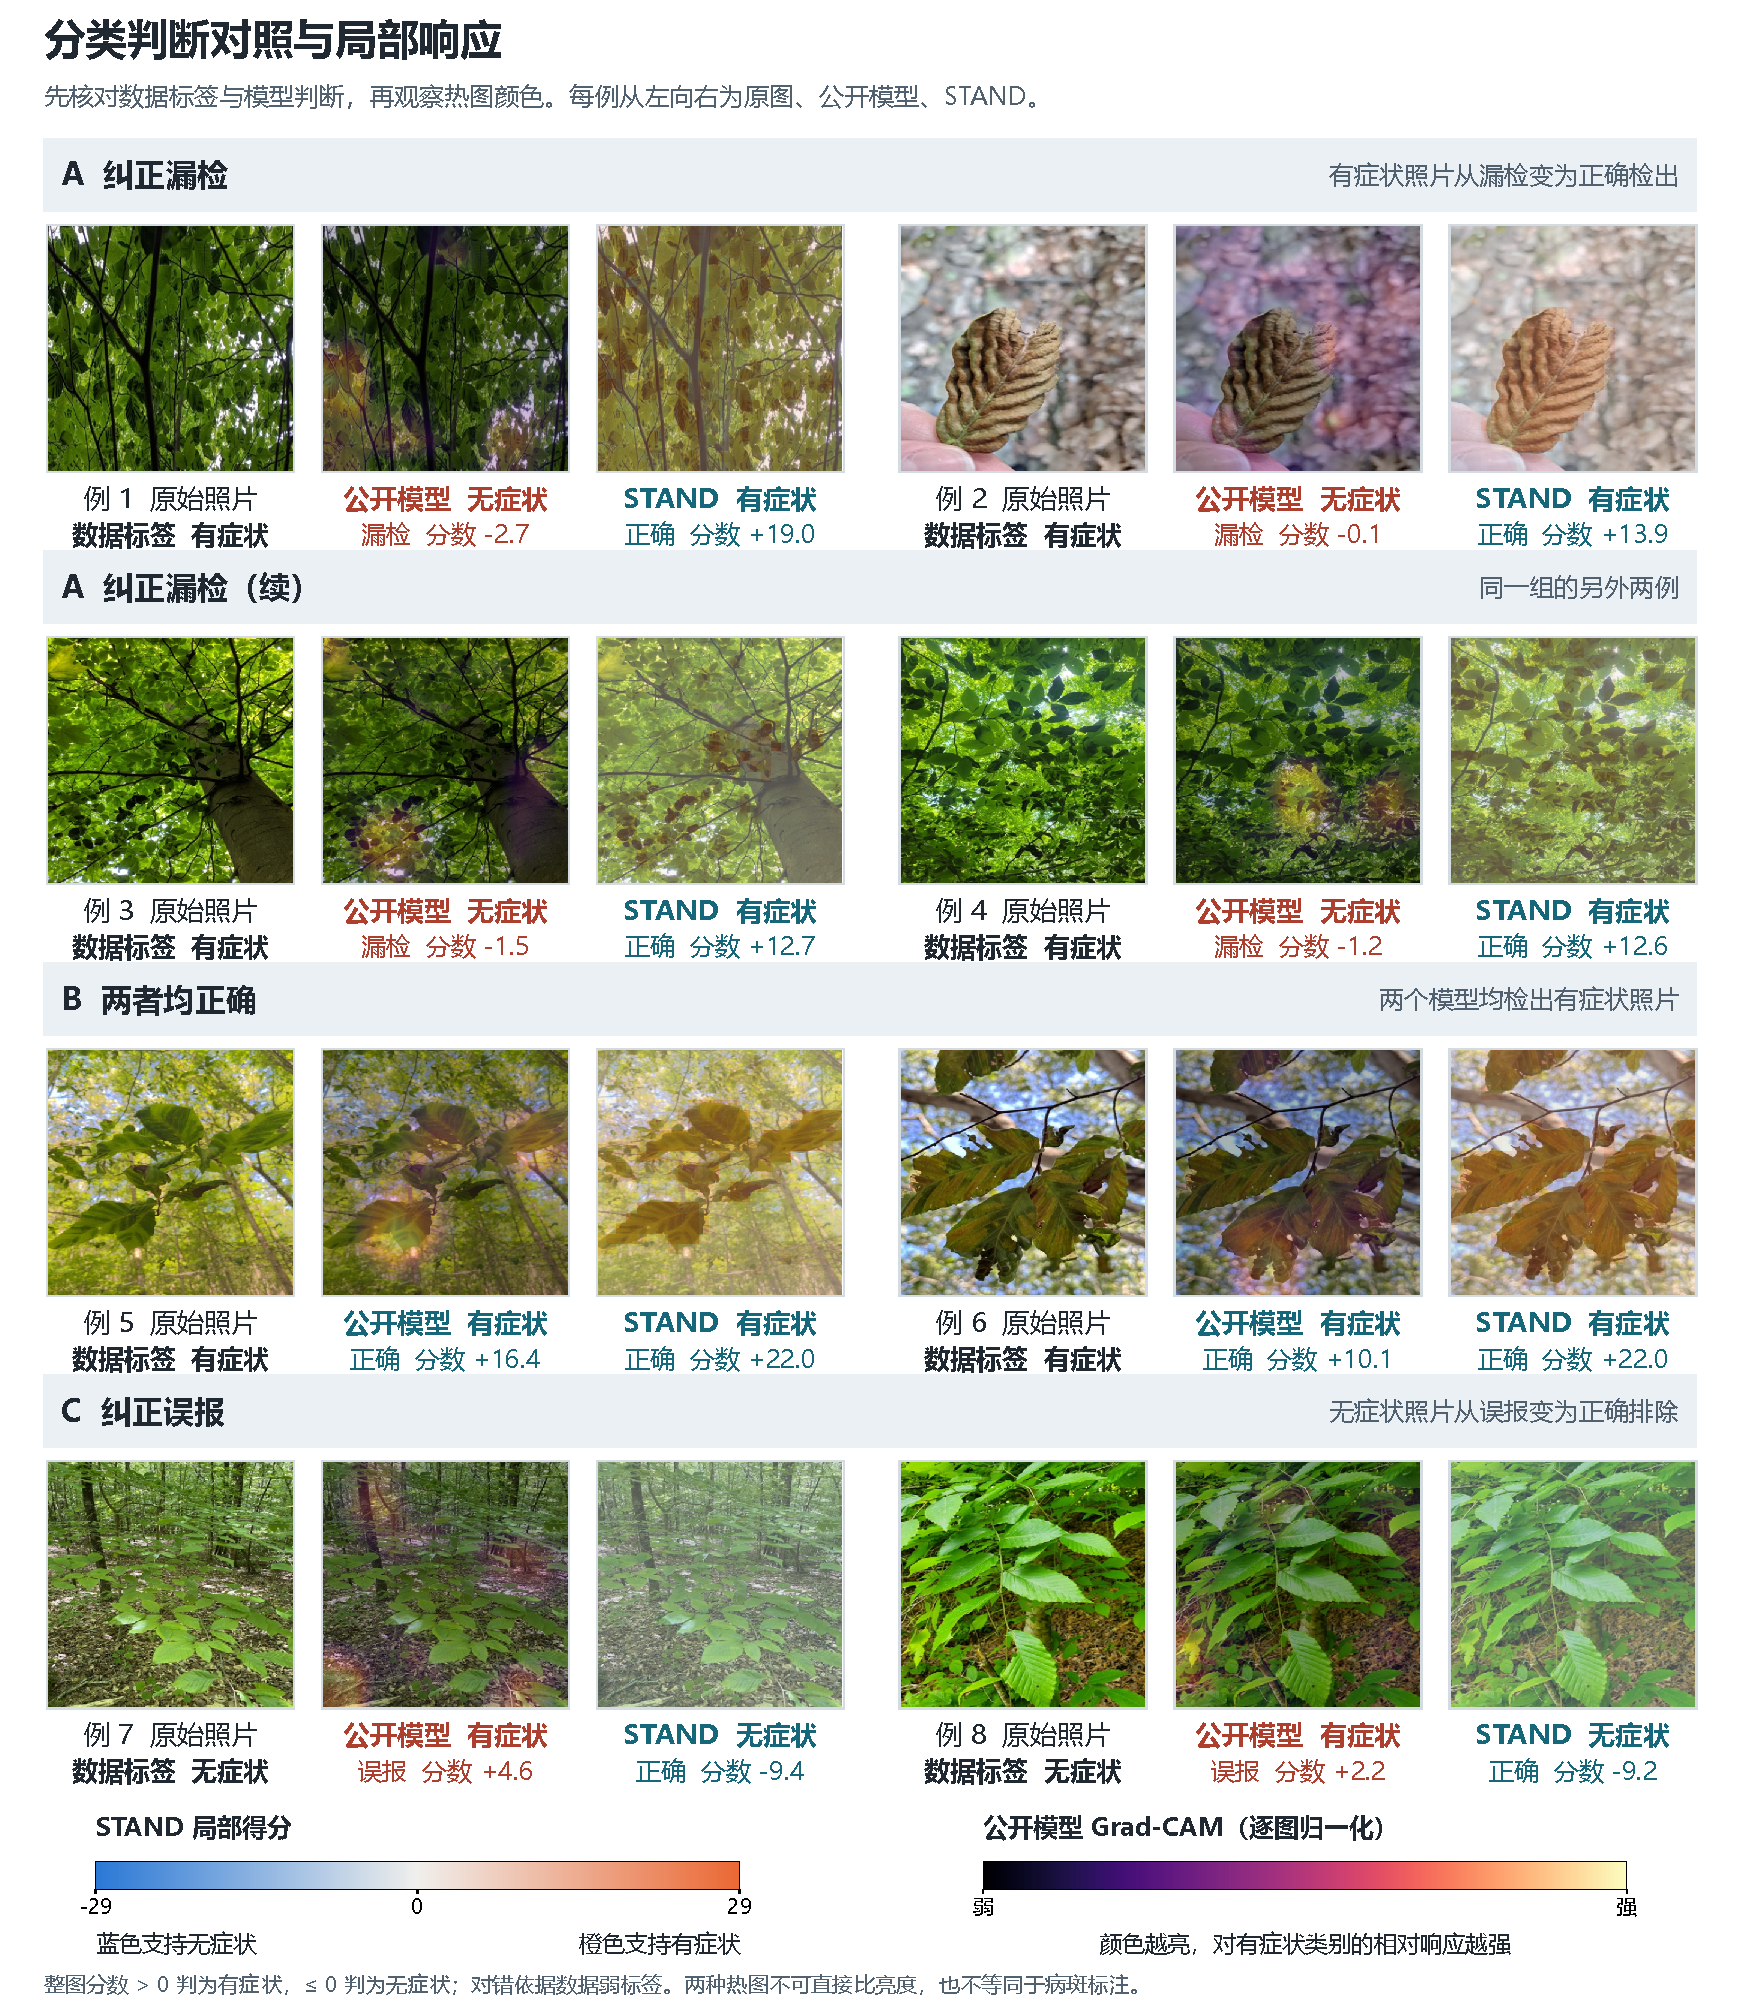
\includegraphics[width=1.0\linewidth,height=.82\textheight,keepaspectratio]{fig18_localisation.pdf}
\caption{STAND 与公开模型的分类判断及局部响应。每例从左到右为原图、公开 EfficientNetV2-S 的 Grad-CAM 和 STAND 热图。A、B、C 分别展示纠正漏检、两者均正确和纠正误报。图中标明数据标签、预测类别与判定结果。STAND 的蓝色与橙色分别支持无症状与有症状，公开模型的亮色表示较强的相对有症状类别响应。对错依据数据弱标签，热图不等同于病斑标注。照片来源与许可见表~\ref{tab:credits}。}
\label{fig:maps}
\end{figure}

区域响应的解释也需要结合错误预测，以区分较强的模型响应与正确的症状判断。漏检样例包含多叶片绿色场景，误报样例可见黄褐色叶片和复杂背景，部分错误预测还具有较大的分数绝对值（图~\ref{fig:fail}）。这些现象说明，症状相关外观仍可能与自然颜色和取景变化混淆。与图~\ref{fig:maps} 中的纠正案例联合观察，能够检查模型使用的区域线索及其不可靠情形。局部响应因此适合作为复核材料，与整图预测、原始照片和标签来源共同使用。

\begin{figure}[htbp]
\centering
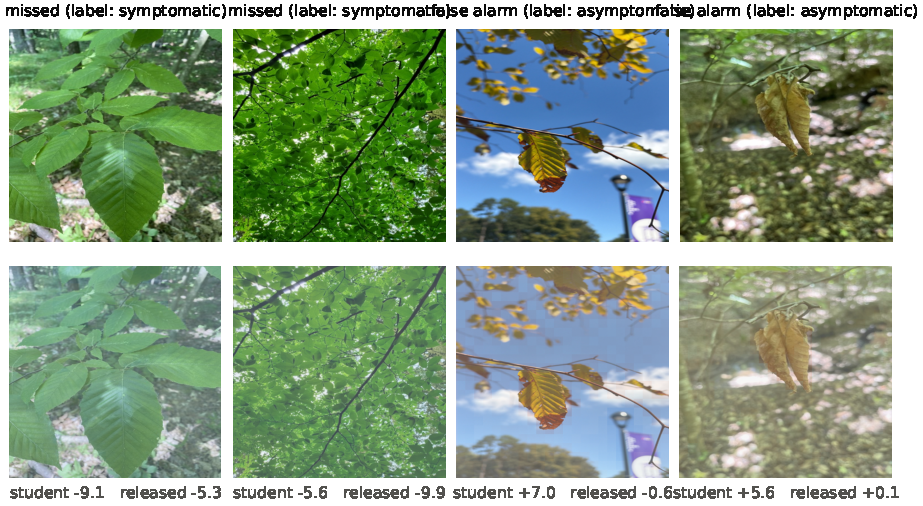
\includegraphics[width=.82\linewidth,height=.74\textheight,keepaspectratio]{fig22_failures.pdf}
\caption{STAND 的漏检与误报案例。第一行为照片，第二行为学生图像块得分。图中标注采用当前弱标签，数字表示学生与公开模型的 logit。热图显示局部分类响应。}
\label{fig:fail}
\end{figure}

\FloatBarrier

\section{讨论}
\label{sec:discussion}
\subsection{从源域表征到目标域决策的互补}
实验结果验证了全局—局部判别与目标分类器适应的互补作用。局部融合主要提高正类检出，单全局学生的消融也显示区域信息在适应后仍有贡献。学生阶段继续改善 AUC 和准确率，说明目标照片参与学习后，同一冻结表征能够产生更合适的排序与决策。AUC 的变化不能由移动教师阈值解释，支持目标分类器重新学习的作用。这些结果共同支持本文保留编码器、融合不同尺度信息并利用独立目标池更新分类规则的设计。

STAND 根据初始教师的预测比例确定两类伪标签的选样数量。它与固定配额的性能差距在低病害来源占比时扩大，验证了调整选样数量可以缓解对称配额在偏斜数据中的限制。两轮训练在配额不变时仍获得改善，说明重新选择照片和更新分类头也是适应的组成部分。极端单一来源下两种配额均下降，则表明选样规则必须有足够的来源和类别覆盖作为基础。组成实验因此同时支持按池分配伪标签的有效性，并说明这一规则不能替代数据多样性。

\subsection{公众监测所需的数据组织}
采集诊断和学习曲线表明，图像数量与采集覆盖对教师学习具有不同影响。时间和设备代理揭示了连续照片中的标签关联，增加采集批次覆盖则改善了跨来源判别。这说明扩充标注数据时需要增加设备、拍摄者、地点和症状外观的变化，而不只增加相同采集条件下的照片。源域标注用于建立症状判别，目标池补充应用来源的特征分布，两类数据共同支持 STAND 的跨来源适应。

主表中的召回率和精确率表明，目标池学习提高了正类检出，同时保持较好的报阳质量，支持将已有标注知识用于公众照片筛查。局部响应允许复核者查看参与判断的区域，困难案例则说明仍需结合原图及标签来源判断其含义。完整系统因而既提供图像级分类，也保留区域响应供复核使用，实际应用可依据漏检与误报成本选择决策阈值。

\subsection{局限与后续验证}
外部标签由平台鉴定和地域规则构成，当前结果衡量给定弱标签与内容筛选条件下的照片识别表现。地域、物种背景和照片内容可能与类别共同变化。拍摄者隔离可避免同一拍摄者的照片同时出现在不同划分中。树木、地点和时间的完全隔离还需要相应的身份和采集记录。后续采用统一专家阅片或病原检测，并预先设计地点和时间留出，将有助于把现有跨来源识别证据推进到诊断一致性评价。

开发阶段曾查看部分外部测试结果，选样规则也受到来源比例实验的启发。现有结果应结合这一开发过程解释。现有区间只描述固定模型的采样变化，未覆盖模型选择偏差。新的确认性评价可预先固定适应规则，采集独立地点、时间与拍摄者照片，并补充症状复核。基础编码器的预训练图像还可能与公众平台照片重合。登记采集时间和图像来源，可为后续数据独立性审计提供依据。

当前主表评价完整系统，CNN 与冻结方法的预训练和监督拟合预算不同。同一编码器、同一数据预算下与 AdaContrast、FreeMatch、MSUN 及冻结多骨干融合的直接比较尚未开展。新增 DINOv2 与 SigLIP~2 对照采用源域线性探测，与 STAND 的预训练数据和目标池使用条件不同。它们补充近期表征基线，但不替代相同骨干下的域适应方法比较。局部学生在训练与评分阶段使用不同统计量，“全局用源域统计、局部用选样统计”配置的测试 AUC 为 97.31、略高于主配置，其变化同时涉及两个分支，完整对照见表~\ref{tab:student_settings}。后续可围绕统一预算对照和逐项标准化控制展开，使现有框架级收益得到更细致的机制解释。

现有实证覆盖 BLD 和当前采集条件。局部热图是经过选样的定性材料，两种响应图的量纲不同。由于缺少病灶掩膜，目前尚未定量评价定位精度。预测概率描述与当前弱标签频率的一致性，其含义不同于病原感染风险。单一来源占比很高的实验包含的重复较少，分层结果亦以描述性比较呈现。补充病灶标注、多病害数据、更多来源比例实验的重复及现场延迟和能耗测量，可分别拓展局部解释、适用范围和部署评价。

\section{结论}
\label{sec:conclusion}
本文提出 STAND，在固定视觉编码器的条件下结合全局—局部分类与独立无标签照片池上的学生学习。局部聚合实验验证了区域响应对整图判断的补充作用，教师—学生对照验证了目标池训练对排序和分类决策的改善。按教师预测比例选样在来源偏斜时优于两类等量选样，两轮重选则在相同配额下提高了目标照片的利用效果。STAND 在按拍摄者隔离的外部测试中取得 91.38\% 准确率和 97.25 的 AUC。实验结果支持通过冻结表征上的分类器适应改善公众照片识别，并说明目标池的来源覆盖是维持适应效果的重要条件。

\section*{数据与研究材料}
源域图像及公开 BLD 模型的出处为 Waldo 等\cite{waldo2026}。外部照片来源于 iNaturalist 的开放许可观察记录。随附工程保留图像清单、拍摄者划分、源域采集批次划分、训练配置、逐图预测及汇总表，可用于核查本研究的数值。公众照片的权利归各原始贡献者所有，使用时应保留对应观察记录及许可信息。


\FloatBarrier
\begingroup
\small\linespread{1.0}\selectfont
\setlength{\bibsep}{4pt}
\bibliographystyle{unsrtnat}
\bibliography{references_recent}
\endgroup

\clearpage
\appendix
\section*{补充材料}
\section{采集关联与评估协议的补充证据}
\subsection{时间与设备分布}
采集批次隔离的必要性首先来自类别与采集条件的关联。按拍摄日和设备统计后，部分组合仅包含一个类别，具体构成见表~\ref{tab:daydev}。在这类数据中，同条件照片增加既可能补充症状样本，也可能重复提供来源线索，随机图像留出难以区分两种作用。完整采集批次及日—设备留出将共享条件从训练和测试两侧分开，使评价转向条件改变后保留的判别能力。数据分布由此解释了分组设置的针对性，也为分类头使用采集批次信息提供了依据。

\begin{table}[htbp]
\centering\small
\caption{源域按拍摄日与设备统计的类别数量。日期为 2025 年月—日，计数用于描述采集组成。}
\label{tab:daydev}
\begin{adjustbox}{max width=\linewidth}
\begin{tabular}{lrrr}
\toprule
日期与设备 & 有症状 & 无症状 & 类别构成\\
\midrule
05-08 iPhone & 0 & 83 & 仅负类\\
06-10 Nikon & 164 & 309 & 两类均有\\
06-11 Nikon & 113 & 0 & 仅正类\\
06-12 Nikon & 0 & 291 & 仅负类\\
06-13 Nikon & 0 & 125 & 仅负类\\
06-13 iPhone & 442 & 201 & 两类均有\\
06-16 Nikon & 68 & 138 & 两类均有\\
\bottomrule
\end{tabular}
\end{adjustbox}
\end{table}


日和设备仍是较粗的采集单位，同一组合内部还可能包含更连续的拍摄过程。将照片按时间展开后，可以观察到连续的单类别采集段，分布见图~\ref{fig:timeline}。相邻照片可能反复呈现相近的叶片和取景，因此即使日—设备标签不变，局部采集条件也具有时间结构。本文按时间连续性定义采集批次，把这种关联用于验证分组和差异估计。该观察说明使用完整采集序列比单独使用设备标签更贴近需要控制的共享条件。

\begin{figure}[htbp]
\centering
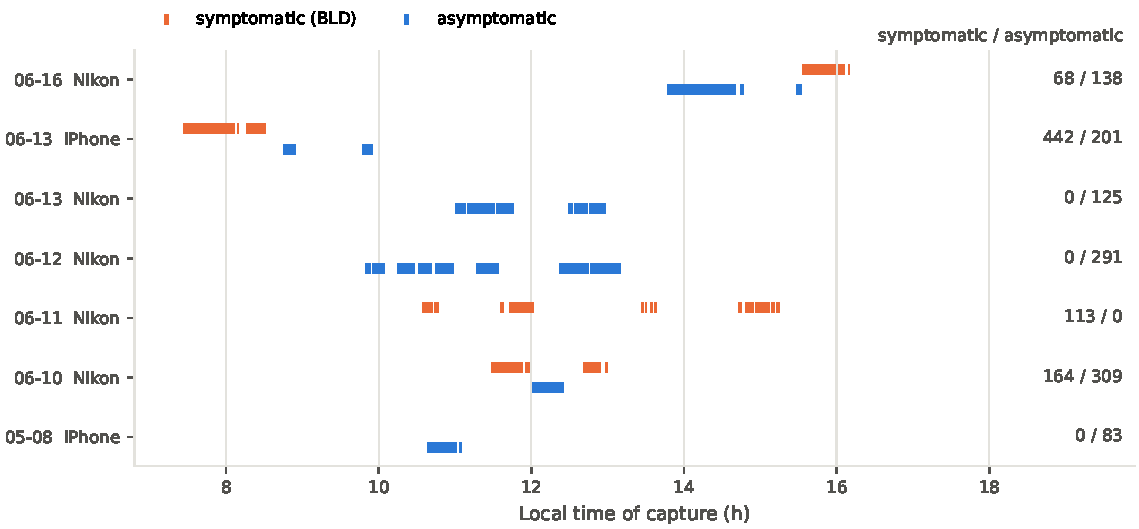
\includegraphics[width=1.0\linewidth,height=.74\textheight,keepaspectratio]{fig02_timeline.pdf}
\caption{源域照片的拍摄时间分布。每行为一个日—设备组合，每个标记是一张照片。右侧为正、负类数量。横轴为本地拍摄小时。}
\label{fig:timeline}
\end{figure}

\subsection{采集代理预测与训练—测试重叠}
采集条件与标签相关，还不足以判断分类器是否能利用这些条件完成预测。我们因而设计简单输入对照，分别使用时间、设备和缩略图等信息，以检查不依赖充分症状细节时能够获得的成绩。仅输入拍摄时间也取得很高的随机划分准确率，缩略图则在采集批次留出后明显下降（表~\ref{tab:probes}）。这验证了采集代理确实具有预测能力，并说明粗略颜色和形状对来源变化敏感。冻结视觉表征在采集批次留出中仍保留较强判别，支持其包含超出简单代理的可迁移信息，也支持采用分组评价检验这种信息。

\begin{table}[htbp]
\centering\small
\caption{采集关联诊断（\%）。前四行使用非图像元数据，缩略图保留粗略颜色和形状，DINOv3 为冻结视觉表征对照。各列最高值加粗。代理预测准确率反映采集信息与标签的关联，AUC 小于 50 表示预测方向在采集批次间反转。}
\label{tab:probes}
\begin{adjustbox}{max width=\linewidth}
\begin{tabular}{lrrrr}
\toprule
输入 & 随机准确率 & 随机 AUC & 采集批次准确率 & 采集批次汇总 AUC\\
\midrule
仅拍摄时间 & 99.07 & 99.96 & 75.13 & 82.70\\
相机元数据与时间 & \textbf{99.69} & \textbf{99.99} & 64.22 & 61.99\\
不含时间的相机元数据 & 75.08 & 78.20 & 33.92 & 19.10\\
仅设备标识 & 67.48 & 64.11 & 48.91 & 51.93\\
单像素平均颜色 & 68.05 & 71.14 & 47.21 & 43.33\\
$4\times4$ 缩略图 & 82.32 & 89.57 & 40.64 & 36.19\\
$8\times8$ 缩略图 & 84.28 & 91.11 & 44.47 & 40.48\\
冻结 DINOv3 全局特征 & 99.28 & 99.93 & \textbf{86.19} & \textbf{95.73}\\
\bottomrule
\end{tabular}
\end{adjustbox}
\end{table}


对相同输入更换验证协议，可以检查其预测信息是否跨采集条件保留。简单代理与冻结视觉表征在随机划分下都表现较好，采集批次留出后两者的差距则增大，比较见图~\ref{fig:probes}。这种变化说明单一随机成绩容易混合评价症状信息和共享采集线索，分组测试则更能区分其迁移能力。本文据此以新采集批次表现检查教师，再以独立拍摄者测试检查目标适应，使两个阶段的评价都对应实际会变化的采集条件。

\begin{figure}[htbp]
\centering
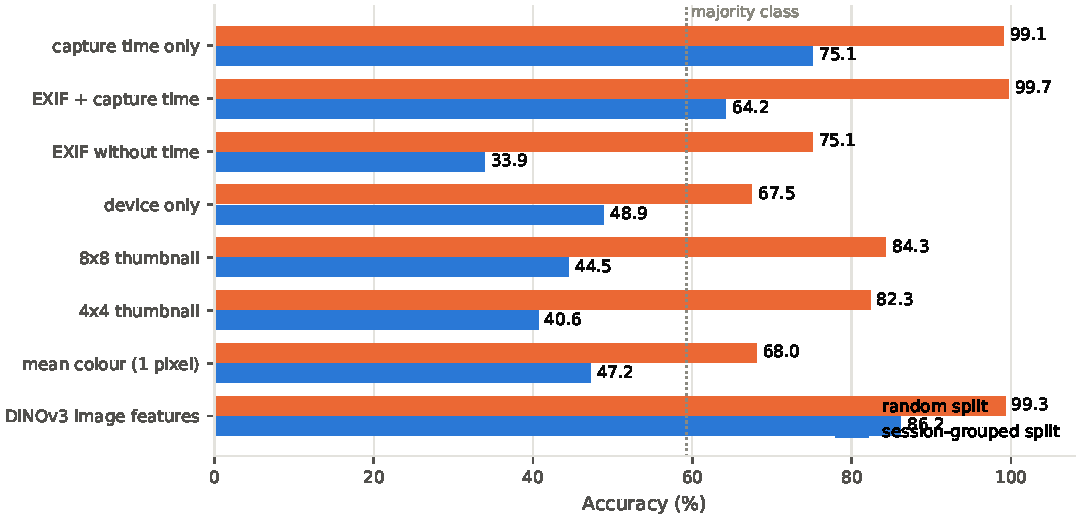
\includegraphics[width=1.0\linewidth,height=.74\textheight,keepaspectratio]{fig03_shortcut_probes.pdf}
\caption{简单输入的随机与采集批次评估准确率。元数据代理不读取图像。缩略图仍保留粗略视觉信息。虚线为多数类参照，DINOv3 行是视觉表征对照。}
\label{fig:probes}
\end{figure}

简单时间代理的有效性可以从训练与测试之间的采集重叠得到解释。所有测试照片均能在训练侧找到同采集批次照片，大量样本还共享短连拍序列，统计结果见表~\ref{tab:leak}。在这种条件下，时间最近邻可通过复制相邻照片标签完成代理预测，而不需要逐张识别症状。不同随机种子都保留了这一结构，说明重新随机划分并不能消除共享采集条件。完整采集批次留出因而是针对性的控制，用于检验表征在连续拍摄关系之外保留的分类能力。

\begin{table}[htbp]
\centering\small
\caption{五次随机划分中的训练—测试采集关系。间隔单位为秒，其余数值为百分数。粗体标示准确率列中最强的采集代理预测，重叠比例与时间间隔用于描述采集联系。}
\label{tab:leak}
\begin{adjustbox}{max width=\linewidth}
\begin{tabular}{lrrrrrrr}
\toprule
种子 & \makecell{共享\\采集批次} & \makecell{共享\\连拍} & \makecell{中位\\间隔} & \makecell{10 秒\\以内} & \makecell{时间近邻\\准确率} & \makecell{特征近邻\\准确率} & \makecell{特征近邻\\共享采集批次}\\
\midrule
0 & 100.00 & 70.10 & 6.00 & 66.67 & \textbf{100.00} & 98.97 & 91.41\\
1 & 100.00 & 75.95 & 5.00 & 71.48 & \textbf{100.00} & 97.94 & 91.75\\
2 & 100.00 & 76.29 & 5.00 & 71.82 & \textbf{100.00} & \textbf{99.31} & 91.07\\
3 & 100.00 & 76.98 & 5.00 & 75.26 & \textbf{100.00} & 96.56 & 90.38\\
4 & 100.00 & 72.51 & 6.00 & 68.73 & \textbf{100.00} & 98.28 & 87.29\\
\bottomrule
\end{tabular}
\end{adjustbox}
\end{table}


图像文件不同并不意味着采集条件独立。测试照片与同设备训练照片可能仅相隔数秒，即使像素不完全相同，也可能共享叶片、取景与背景。最近拍摄时间差和连拍共享比例量化了这种关系（图~\ref{fig:leak}），说明文件去重与采集隔离分别控制不同的问题。本文根据采集关系划分完整采集批次，减少连续照片跨训练与测试两侧出现的影响，从而更明确地观察教师在新条件下的判别表现。

\begin{figure}[htbp]
\centering
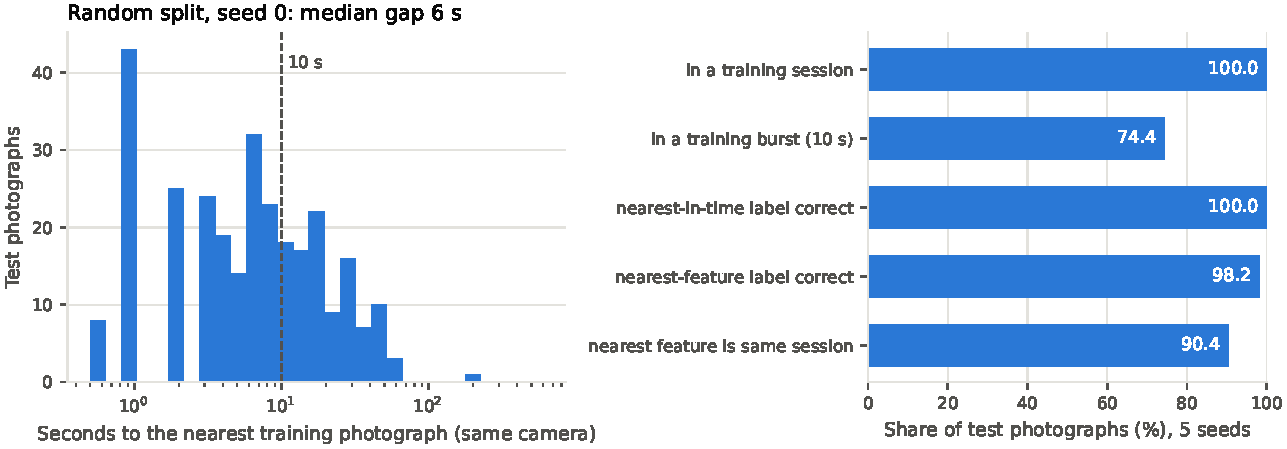
\includegraphics[width=1.0\linewidth,height=.74\textheight,keepaspectratio]{fig04_leakage.pdf}
\caption{随机划分的采集重叠。左为种子 0 下各测试照片到同设备最近训练照片的时间差，右为五次划分的平均比例。“重叠”按采集批次或连拍共享定义。}
\label{fig:leak}
\end{figure}

\subsection{冻结特征中的类别与采集批次结构}
冻结特征可以同时编码症状和采集外观，二者在同一表示中并存会影响投影的对象。为观察这一结构，我们对相同特征分别按类别和采集批次着色，并展示投影后的分布，见图~\ref{fig:pca}。类别与采集批次结构同时存在，说明直接去除总体主方向可能混合处理两类信息。本文先在同类别内计算采集批次均值偏差，再根据分类结果选择投影维数。这一约束对性能的影响见表~\ref{tab:ablk}。可视化与定量对照共同支持将正交投影作为辅助处理，而不将其解释为已经完全分离症状和采集因素。

\begin{figure}[htbp]
\centering
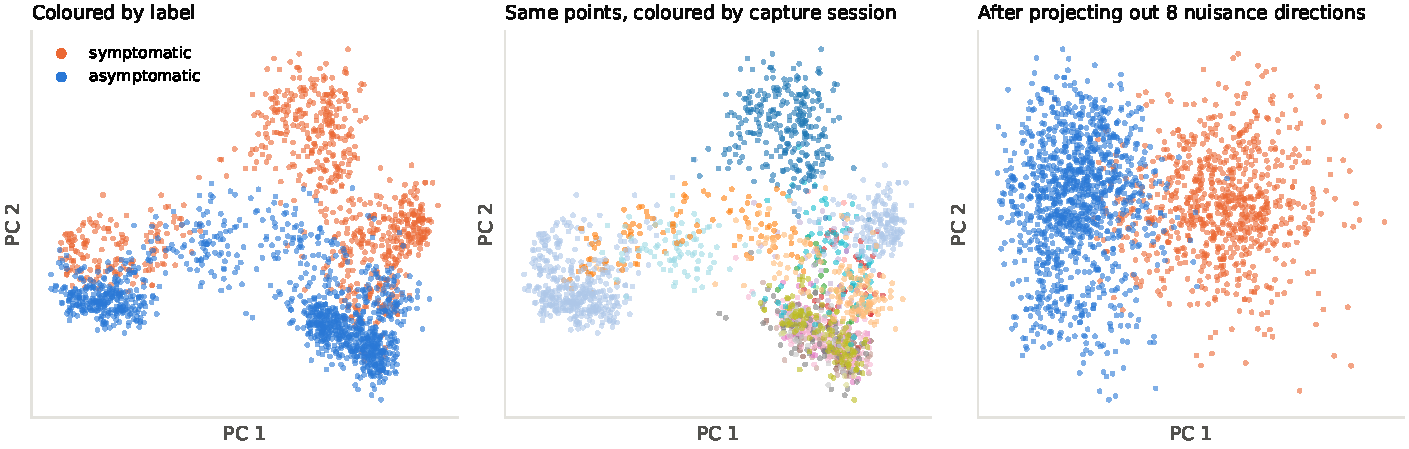
\includegraphics[width=1.0\linewidth,height=.74\textheight,keepaspectratio]{fig24_feature_space.pdf}
\caption{源域冻结全局特征的二维 PCA 可视化。三个面板分别显示类别、采集批次及投影后的类别结构。定量分类结果见正交投影消融。}
\label{fig:pca}
\end{figure}

\FloatBarrier
\section{STAND 教师的补充诊断}
\label{app:teacher}
本节集中检查教师进入学生训练之前的判别基础。采集批次逐折、投影维数、骨干和聚合规则实验分别说明初始化条件及设计选择，完整 STAND 的性能与组件贡献由正文中的共同外部测试和学生消融评价。

\subsection{适应前教师的跨采集批次排序与决策}
源域采集批次留出与公众照片测试考察不同采集条件下的分类表现。L1 的采集批次默认准确率高于 L3，而 L3 在公众照片上表现更好（表~\ref{tab:session} 和表~\ref{tab:ladder}）。这一排名变化说明，源域内部泛化和目标来源表现需要分别评价。分类器适应的收益由同一外部测试上的教师—学生对照检验。


为了判断采集批次间的变化主要影响样本区分还是类别决策，我们同时比较 AUC、默认准确率和无标签阈值调整后的准确率。L3 的采集批次平均 AUC 为 98.53，默认准确率为 80.97\%。利用待测折的无标签分数调整阈值后，准确率达到 93.69\%（表~\ref{tab:session}）。较强的排序与明显的阈值收益同时存在，说明部分判别信息已保留在分数中，但固定决策位置尚未充分利用它。日—设备留出也显示局部融合在更大采集单元变化下保留了判别能力。这些结果支持将教师排序用于伪标签选择，再由目标分布帮助形成分类决策。

\begin{table}[htbp]
\centering\small
\caption{适应前教师与源域分类器的分组诊断（\%）。L1--L3 为 STAND 的教师构建阶段。采集批次 AUC 为逐折平均值，准确率为合并折外预测后的指标。调整阈值读取待测折无标签分数，属于转导诊断。日—设备列为七组留一准确率。CNN 与冻结头的拟合样本预算不同。粗体表示各列最高值。}
\label{tab:session}
\begin{adjustbox}{max width=\linewidth}
\begin{tabular}{lrrrr}
\toprule
方法 & \makecell{采集批次默认\\准确率} & \makecell{采集批次逐折\\平均 AUC} & \makecell{采集批次调整\\阈值准确率} & \makecell{日—设备\\准确率}\\
\midrule
EfficientNetV2-S\cite{tan2021} & 73.84 & 86.94 & 78.44 & ---\\
Inception-v3\cite{szegedy2016} & 80.82 & 86.46 & 80.82 & ---\\
MobileNetV3-Large\cite{howard2019} & 80.82 & 91.90 & 83.92 & ---\\
ResNet-50\cite{he2016} & 69.44 & 78.74 & 74.92 & ---\\
L1 冻结全局分类 & \textbf{86.19} & 97.48 & 91.62 & 88.16\\
L2 加入正交投影 & 84.75 & 97.63 & 90.43 & 88.73\\
L3 STAND 教师（未适应） & 80.97 & \textbf{98.53} & \textbf{93.69} & \textbf{89.97}\\
\bottomrule
\end{tabular}
\end{adjustbox}
\end{table}


平均成绩可能掩盖不同采集批次之间的差异，教师用于选样时尤其需要稳定的排序作为基础。我们因而将五折结果分别展开，比较每折的 AUC 与调整阈值后的准确率。L3 各折 AUC 均不低于 97.32，说明较强的判别能力在不同采集批次中均有体现。准确率仍随采集批次变化，表明排序与最终决策对采集条件的敏感性不同（图~\ref{fig:folds}）。各折排序结果为采用教师分数两端选样提供了诊断依据。选样后能否改善新照片的分类，由正文表~\ref{tab:ablation} 中完整 STAND 与未适应教师的同测试集对照检验。

\begin{figure}[htbp]
\centering
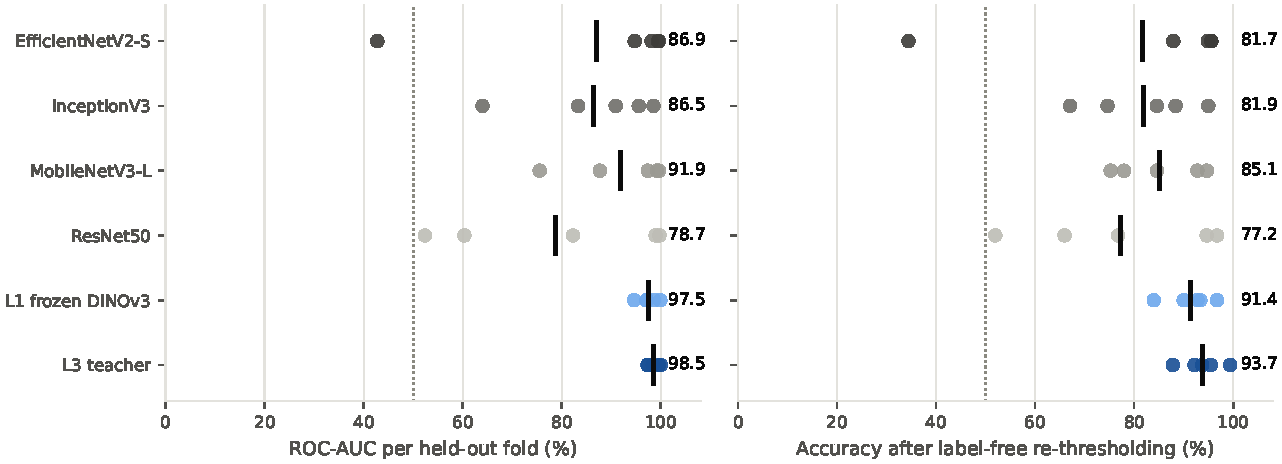
\includegraphics[width=1.0\linewidth,height=.74\textheight,keepaspectratio]{fig07_session_folds.pdf}
\caption{适应前分类器的采集批次留出各折结果。L3 为 STAND 的全局—局部教师。本图未执行独立目标池学生适应。点代表单折，条形为五折算术平均。左侧为 AUC，右侧为读取待测折分数后调整阈值的准确率。完整默认阈值结果见表~\ref{tab:perfold}。}
\label{fig:folds}
\end{figure}

源域 23 个采集批次中有 21 个仅包含单一类别，类别与采集条件因而经常同时变化。若将连续照片随机分到训练和测试两侧，共享的采集信息也可能被用于预测。附录图~\ref{fig:timeline}--\ref{fig:leak} 及表~\ref{tab:probes}--\ref{tab:leak} 的代理实验验证了这种关联。采集批次隔离用于检验教师在新采集条件下的判别能力，拍摄者隔离用于检验目标池学习对新来源的迁移效果，两种划分共同约束了本文的跨来源结论。

\subsection{教师投影的维数与方向}
正交投影的强度决定保留多少原始特征方向。同类采集批次均值的差异可能同时包含采集条件和症状外观，因此投影维数应根据分类表现选择，而不能只追求移除更多变化。维数对照中，$k=16$ 获得最高外部 AUC，但并非默认准确率最优配置，源域采集批次和公众照片也偏好不同维数（表~\ref{tab:ablk}）。这说明投影对排序和决策的影响并不一致。训练内选出的 $k=8$ 相对不投影提高了外部准确率，支持将采集批次信息作为可调的辅助约束。直接面向目标分布的分类器更新仍由学生阶段承担。

\begin{table}[htbp]
\centering\small
\caption{正交投影维数与全局分类头正则化消融（\%）。上区固定 $C=0.1$。下区使用嵌套选择的投影维数。外部主配置为 $k=8$。各区分别加粗列最高指标。}
\label{tab:ablk}
\begin{adjustbox}{max width=\linewidth}
\begin{tabular}{lrrrrr}
\toprule
设置 & \makecell{采集批次逐折\\AUC} & \makecell{采集批次调整\\阈值准确率} & 外部 AUC & 外部准确率 & \makecell{外部调整\\阈值准确率}\\
\midrule
\multicolumn{6}{l}{\textit{投影维数}}\\
\addlinespace[2pt]
$k=0$ & 97.48 & 91.62 & 94.02 & 80.60 & 86.75\\
$k=1$ & 97.47 & 91.73 & 93.76 & 79.74 & 86.31\\
$k=2$ & 96.55 & 91.42 & 93.62 & 80.23 & 86.31\\
$k=4$ & \textbf{98.24} & 93.69 & 94.49 & 82.60 & 86.96\\
$k=8$ & 98.19 & \textbf{93.90} & 94.42 & 83.41 & 87.18\\
$k=12$ & 97.63 & 91.73 & 94.94 & \textbf{83.57} & 88.04\\
$k=16$ & 97.56 & 90.18 & \textbf{95.60} & 80.82 & \textbf{88.47}\\
$k=24$ & 97.56 & 89.81 & 95.01 & 80.71 & 87.93\\
嵌套验证选择 $k$（主配置） & 97.63 & 90.43 & 94.42 & 83.41 & 87.18\\
\midrule
\multicolumn{6}{l}{\textit{正则化强度}}\\
\addlinespace[2pt]
$C=0.001$ & 97.25 & \textbf{92.40} & 92.80 & 82.87 & 82.87\\
$C=0.01$ & 97.52 & 91.88 & 94.18 & \textbf{83.41} & 85.94\\
$C=0.1$（主配置） & \textbf{97.63} & 90.43 & 94.42 & \textbf{83.41} & \textbf{87.18}\\
$C=1$ & \textbf{97.63} & 89.92 & 94.11 & 82.11 & 86.75\\
$C=10$ & 97.23 & 89.56 & \textbf{94.59} & 80.55 & \textbf{87.18}\\
\bottomrule
\end{tabular}
\end{adjustbox}
\end{table}


投影方向的方差解释率衡量采集批次差异在特征空间中的集中程度，分类指标则检验移除这些方向后剩余信息是否仍有用。将二者并列可以区分统计变化与任务收益。采集批次差异主要集中在少数方向，但内部和外部 AUC 均不随移除维数单调提高（图~\ref{fig:nuisance}），说明高方差方向并不全是无关信息。本文先在同类别内部估计采集批次偏差，再用训练内分组验证选择维数，以限制对症状判别信息的损失。方差与性能之间的差异支持有选择地约束采集变化，也说明投影应作为辅助处理使用。

\begin{figure}[htbp]
\centering
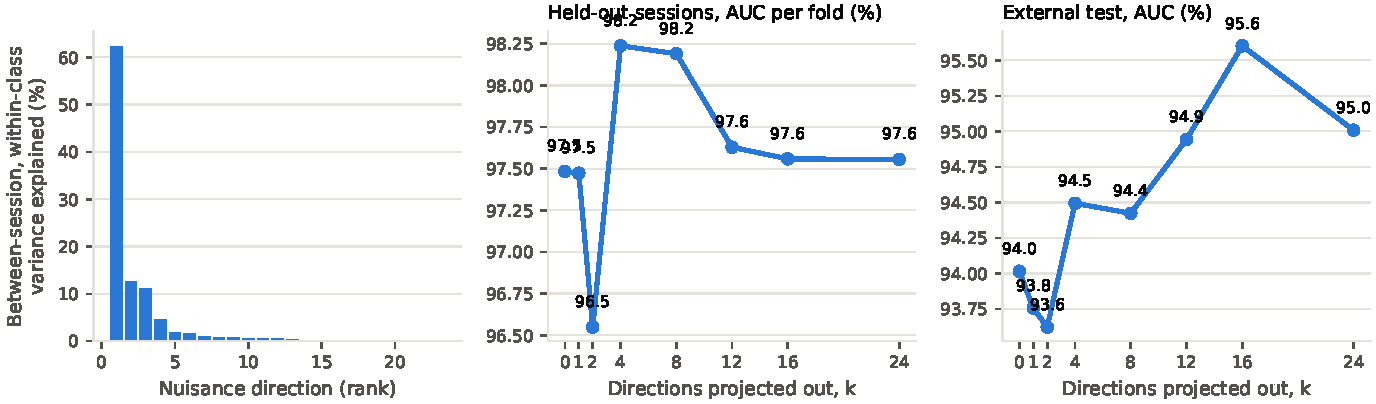
\includegraphics[width=1.0\linewidth,height=.74\textheight,keepaspectratio]{fig12_nuisance.pdf}
\caption{适应前教师的正交投影方向及维数敏感性。三个面板从左至右依次为同类别采集批次均值差异的方差解释率、采集批次逐折平均 AUC 和外部 AUC。横轴为移除的同类采集批次差异方向数。}
\label{fig:nuisance}
\end{figure}

\subsection{教师初始化的表征选择}
冻结编码器的前提是已有表征能够为病害分类提供足够信息。为检查这一前提，我们在相同全局分类头范式下比较不同预训练骨干，使差异主要反映可供分类头利用的特征。自监督 DINO 表征整体优于所比较的冻结 ImageNet CNN 表征，验证了仅训练轻量分类头也可获得较强的任务判别能力（表~\ref{tab:backbone}）。其中，DINOv2-B/14 取得最高外部 AUC，DINOv3-B/16 主配置取得最高默认准确率，说明表征对排序和决策的影响有所不同。该结果支持复用已有视觉特征，而 STAND 的局部融合与适应收益由共享编码器的组件实验单独检验。

\begin{table}[htbp]
\centering\small
\caption{同类全局分类头下的表征与分辨率比较（\%）。$k$ 由训练内验证选择，模型配置依据源域采集批次结果确定，外部列用于迁移分析。各列最高值加粗。}
\label{tab:backbone}
\begin{adjustbox}{max width=\linewidth}
\begin{tabular}{lrrrrr}
\toprule
设置 & \makecell{采集批次逐折\\AUC} & \makecell{采集批次调整\\阈值准确率} & 外部 AUC & 外部准确率 & \makecell{外部调整\\阈值准确率}\\
\midrule
DINOv3-B/16，384（主配置）\cite{simeoni2026} & 97.63 & 90.43 & 94.42 & \textbf{83.41} & 87.18\\
DINOv3-L/16，384 & \textbf{98.01} & 89.87 & 92.36 & 80.60 & 82.97\\
DINOv3-S/16，384 & 97.14 & 90.74 & 92.49 & 82.49 & 83.89\\
DINOv3 ConvNeXt-S，384 & 91.16 & 81.08 & 86.90 & 62.72 & 76.13\\
DINOv2-B/14，392\cite{oquab2024} & 95.46 & 89.66 & \textbf{96.66} & 80.12 & \textbf{90.41}\\
DINOv3-B/16，224 & 95.44 & 87.38 & 94.94 & 80.01 & 87.39\\
DINOv3-B/16，512 & 97.92 & \textbf{92.66} & 95.04 & 82.97 & 87.98\\
DINOv3-B/16，图像块均值 & 96.42 & 88.06 & 88.23 & 78.29 & 79.74\\
冻结 EfficientNetV2-S\cite{tan2021} & 79.84 & 69.49 & 68.79 & 63.20 & 61.69\\
冻结 ResNet-50\cite{he2016} & 80.79 & 71.61 & 77.28 & 68.59 & 65.30\\
\bottomrule
\end{tabular}
\end{adjustbox}
\end{table}


较大的骨干或更高的源域成绩并不必然意味着公众照片上的决策更准确。源域拟合与目标来源的差异还会影响表征的使用方式，因此需要同时观察两个评价来源。DINOv3-L 的源域采集批次排序较好，外部全局头却弱于主配置。改变输入尺度也会改变两侧表现，形成不同的模型排名（图~\ref{fig:backbone}）。这一现象说明，模型容量和目标决策适配是两个相互关联的因素。本文固定编码器后显式学习目标分类头，使适应过程直接利用公众照片的特征分布，而不将跨来源改善完全寄托于更换骨干。

\begin{figure}[htbp]
\centering
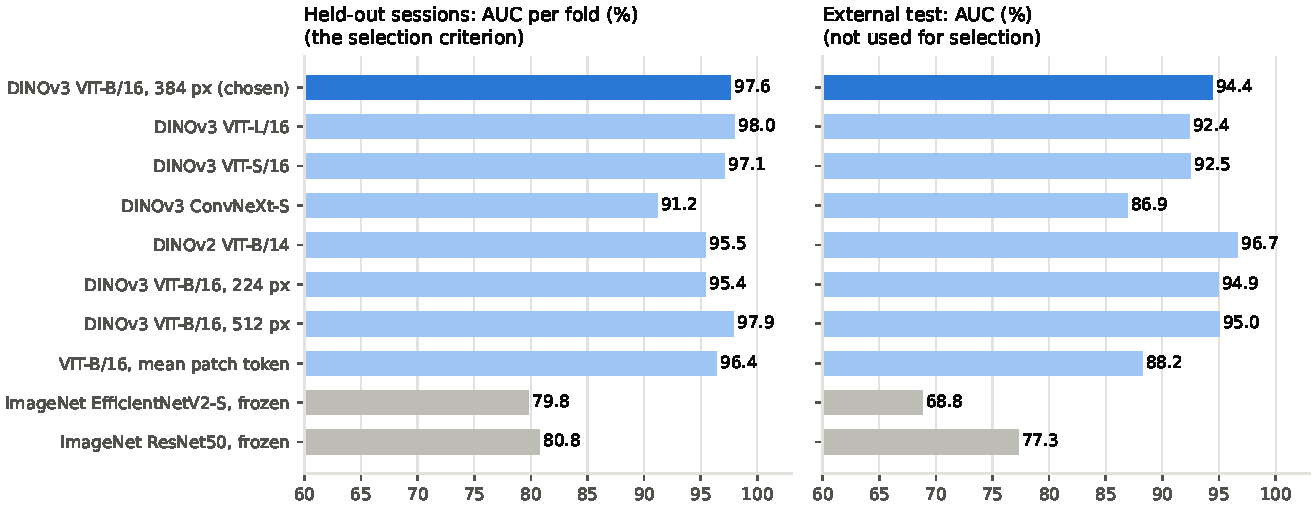
\includegraphics[width=1.0\linewidth,height=.74\textheight,keepaspectratio]{fig13_backbones.pdf}
\caption{教师初始化的冻结表征比较。各配置尚未执行目标池适应。左图为源域采集批次选择依据，右图为外部迁移分析。各配置均采用对应的全局分类头。}
\label{fig:backbone}
\end{figure}

\subsection{教师局部分支的聚合选择}
局部分支需要把多个区域的响应转换为一张照片的分数。简单均值给予所有位置相同权重，容易弱化较小的高响应区域。最大池化只保留一个峰值，又会丢失其他位置的信息。我们据此比较均值、最大值和 log-mean-exp 聚合，并分别评价单局部头及其与全局头的融合。log-mean-exp 在这些对照中表现较好，全局—局部融合又优于单局部头（表~\ref{tab:pooling}）。这说明提高高响应区域的权重、同时保留多个位置的贡献更有利于图像级分类，也说明区域响应仍需整图信息补充。实验支持在图像级监督下采用平滑局部聚合与全局判别相结合的设计。

\begin{table}[htbp]
\centering\small
\caption{局部分类头的聚合、投影与种子敏感性（\%）。融合 AUC 使用全局与局部的平均分数。各列最高值加粗，包括不同种子的结果。}
\label{tab:pooling}
\begin{adjustbox}{max width=\linewidth}
\begin{tabular}{lrrrrr}
\toprule
设置 & \makecell{采集批次逐折\\AUC} & \makecell{采集批次调整\\阈值准确率} & \makecell{外部融合\\AUC} & \makecell{外部局部头\\AUC} & 外部准确率\\
\midrule
均值 & 97.82 & 90.80 & 92.89 & 88.32 & 82.92\\
log-mean-exp，$\tau=0.3$ & 98.46 & 93.17 & 94.97 & 94.24 & 88.15\\
log-mean-exp，$\tau=1$（主配置） & \textbf{98.53} & 93.69 & 95.09 & 94.29 & 88.36\\
log-mean-exp，$\tau=3$ & 98.48 & 93.69 & 95.00 & 94.05 & 88.09\\
最高 10\% 均值 & 98.31 & 93.02 & 94.46 & 92.85 & 87.88\\
最大值 & 98.29 & 92.86 & 94.76 & 93.32 & 87.88\\
$\tau=1$，不使用投影 & 95.99 & 91.42 & 95.11 & \textbf{94.74} & 87.12\\
$\tau=1$，第二个种子 & 98.49 & \textbf{93.74} & \textbf{95.22} & 94.60 & \textbf{88.58}\\
$\tau=1$，第三个种子 & 98.48 & 93.49 & 95.09 & 94.28 & 88.31\\
\bottomrule
\end{tabular}
\end{adjustbox}
\end{table}


在确定聚合形式后，还需要检查性能是否依赖某一个温度设置。温度控制高分图像块相对其他位置的权重，而不改变分类头结构或训练标签，因此可用于考察局部证据选择的敏感性。按照式~\eqref{eq:mil} 调整温度后，$0.3$、$1$ 和 $3$ 的表现接近，均高于简单均值和最大池化（图~\ref{fig:pooling}）。不同种子也维持相近水平，说明在所测试的范围内，平滑聚合能够持续利用多位置响应。该结果支持聚合形式本身的有效性，而不仅是某个温度或初始化恰好取得较好结果。

\begin{figure}[htbp]
\centering
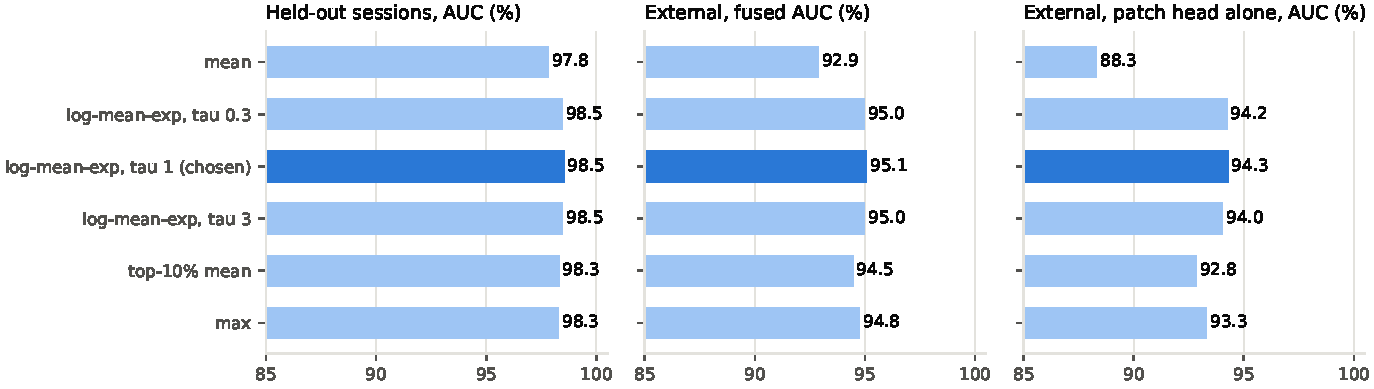
\includegraphics[width=1.0\linewidth,height=.74\textheight,keepaspectratio]{fig14_pooling.pdf}
\caption{适应前教师的局部聚合规则。三个面板从左至右依次为采集批次 AUC、外部全局—局部融合 AUC 和外部单局部头 AUC。所有图像块共享线性打分头。}
\label{fig:pooling}
\end{figure}

\FloatBarrier
\section{逐折细节与固定配额转导诊断}
\subsection{逐折默认阈值结果}
汇总指标中的排序与决策差异，在单个留出折上更加直观。折 1 的 AUC 为 97.32，默认准确率却为 36.02\%，完整结果见表~\ref{tab:perfold}。这说明模型仍能较好地区分正、负样本的相对次序，但固定阈值不适合该折分数分布。由于 AUC 对保持次序的变换不变，这种组合支持把信息是否保留与决策是否适配分开分析。教师仍可从分数两端产生候选伪标签，再由目标照片帮助学习分类规则，为固定编码器的适应提供基础。

\begin{table}[htbp]
\centering\small
\caption{采集批次留出逐折结果。单元格为默认准确率 / AUC（\%）。每折中两种指标分别加粗最高值。每折测试集分别为 485、422、318、370、339 张。表~\ref{tab:session} 的采集批次 AUC 取此处逐折均值。}
\label{tab:perfold}
\begin{adjustbox}{max width=\linewidth}
\begin{tabular}{lrrrrr}
\toprule
模型 & 折 0 & 折 1 & 折 2 & 折 3 & 折 4\\
\midrule
EfficientNetV2-S & 38.56 / 42.77 & \textbf{80.09} / 94.72 & \textbf{97.17} / \textbf{99.44} & 74.32 / 98.15 & 94.10 / 99.62\\
Inception-v3 & 71.55 / 64.01 & 76.54 / 83.33 & 82.70 / 90.89 & 83.24 / 95.55 & 94.99 / 98.54\\
MobileNetV3-Large & 64.54 / 75.56 & 75.59 / 87.69 & 94.03 / 99.20 & 83.24 / 97.38 & 95.58 / 99.65\\
ResNet-50 & 38.14 / 52.37 & 73.46 / 82.28 & 89.94 / 98.95 & 62.97 / 60.34 & 97.05 / 99.74\\
L1 全局头 & 93.61 / 98.60 & 65.40 / 97.09 & 85.85 / 94.62 & 89.19 / 97.21 & 98.53 / 99.90\\
L2 正交投影 & 94.02 / 98.71 & 58.53 / 96.84 & 85.22 / 95.70 & 88.65 / 96.91 & \textbf{99.41} / 99.99\\
L3 全局—局部教师 & \textbf{94.23} / \textbf{99.57} & 36.02 / \textbf{97.32} & 85.53 / 97.40 & \textbf{94.05} / \textbf{98.37} & \textbf{99.41} / \textbf{100.00}\\
\bottomrule
\end{tabular}
\end{adjustbox}
\end{table}


\subsection{直接使用待测采集批次的转导实验}
独立目标池实验检验 STAND 能否用于新的拍摄者，本节则考察直接利用待测采集批次的转导变体。该变体固定选取分数两端各 30\% 的照片，并执行两轮学生训练。该变体采用两类等量选样。正文 STAND 根据教师预测比例确定两类样本数量，并使用独立适应池。我们分别采用阈值修正和学生学习，前者保持原排序，后者重新生成分类分数。阈值修正在折 1 的准确率更高，学生则使五折 AUC 均提高或持平，并取得 94.3\% 的总体准确率（表~\ref{tab:trans}）。两种处理产生不同结果，说明目标数据既可用于调整已有排序的决策位置，也可用于学习新的样本区分。该对照支持分类器重新拟合具有阈值修正之外的作用，同时保留转导评价与外部归纳评价的区别。

\begin{table}[htbp]
\centering\small
\caption{固定配额转导变体的采集批次诊断（\%）。学生在待测折分数两端各选取 30\% 的照片训练两轮，完整 STAND 根据教师预测比例确定两类样本数量，并使用独立适应池。每折照片数 / 正类数为 485/271、422/113、318/117、370/171、339/115。准确率和 AUC 两区内逐列加粗最高值。}
\label{tab:trans}
\begin{adjustbox}{max width=\linewidth}
\begin{tabular}{lrrrrr}
\toprule
模型与指标 & 折 0 & 折 1 & 折 2 & 折 3 & 折 4\\
\midrule
\multicolumn{6}{l}{\textit{决策准确率}}\\
\addlinespace[2pt]
教师 默认准确率 & 94.23 & 36.02 & 85.53 & 94.05 & \textbf{99.41}\\
教师 调整阈值准确率 & 95.46 & \textbf{92.18} & \textbf{93.71} & 87.84 & \textbf{99.41}\\
固定配额学生 默认准确率 & \textbf{99.79} & 83.41 & 90.88 & \textbf{98.65} & 98.23\\
\midrule
\multicolumn{6}{l}{\textit{排序 AUC}}\\
\addlinespace[2pt]
教师 AUC & 99.57 & 97.32 & 97.40 & 98.37 & \textbf{100.00}\\
固定配额学生 AUC & \textbf{99.99} & \textbf{98.72} & \textbf{99.32} & \textbf{99.99} & \textbf{100.00}\\
\bottomrule
\end{tabular}
\end{adjustbox}
\end{table}


适应空间还取决于教师在每个采集批次上的初始状态。默认决策偏移较大的折通常有更多改善空间。折 4 原有的排序已接近完全分离，学生 AUC 保持 100.00，但默认准确率略低，逐折变化见图~\ref{fig:trans}。这说明当排序信息已经充分时，少量样本的归属仍受阈值位置影响，执行更新本身并不保证所有决策指标同步提高。分别检查排序和阈值有助于解释各折收益，也使正文独立照片池的迁移结果具有更具体的内部参照。

\begin{figure}[htbp]
\centering
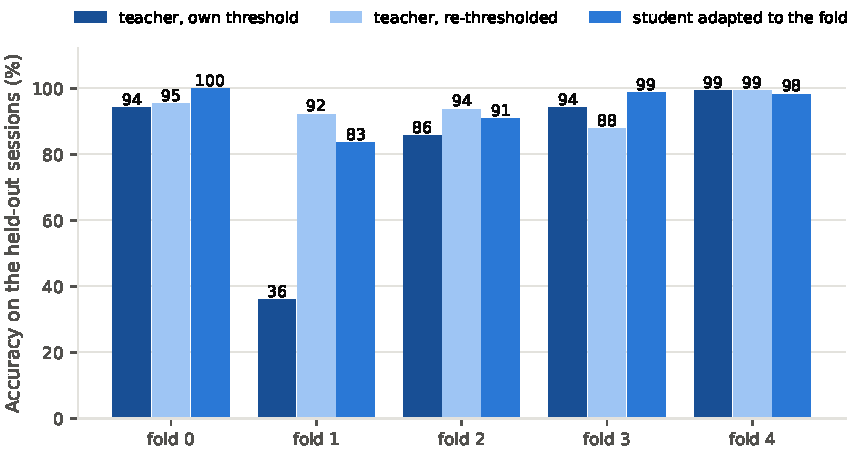
\includegraphics[width=.8\linewidth,height=.74\textheight,keepaspectratio]{fig23_transductive_sessions.pdf}
\caption{采集批次转导适应前后的各折准确率。三组柱分别为同一折的教师默认准确率、教师调整阈值准确率和固定配额转导学生准确率。学生选取分数两端各 30\% 的照片训练两轮，待测折参与拟合。该设置区别于正文完整 STAND。}
\label{fig:trans}
\end{figure}

\FloatBarrier
\section{标注覆盖、实现细节与图片来源}
\subsection{标注数量与采集批次覆盖}
教师训练既需要症状标签，也需要这些标签覆盖足够多的采集条件。为区分数量和覆盖的影响，我们分别按随机图像与完整采集批次组织学习曲线，并保留各自对应的抽样和模型设置。少量随机标签已能在冻结特征上建立有效排序，而采集批次覆盖过少时跨来源表现受到限制，增加覆盖后得到改善（表~\ref{tab:coverage}）。前者验证了预训练表征对教师初始化的作用，后者说明重复采集相近照片不能替代类内外观的多样性。源域数据组织因而需要兼顾标签数量与采集覆盖，为目标池选样提供较好的教师。

\begin{table}[htbp]
\centering\small
\caption{标注数量与采集覆盖实验，AUC 乘以 100。每区加粗平均 AUC 最高值，范围为运行最小值至最大值。各区采用对应模型和独立抽样设置，用于描述各自的资源变化趋势。}
\label{tab:coverage}
\begin{adjustbox}{max width=\linewidth}
\begin{tabular}{lrrr}
\toprule
抽样条件 & 运行次数 & 外部平均 AUC & 运行范围\\
\midrule
\multicolumn{4}{l}{\textit{随机图像 L1（不使用投影）}}\\
\addlinespace[2pt]
25 张 & 3 & 87.79 & 81.91--91.67\\
50 张 & 3 & 87.41 & 85.32--91.06\\
100 张 & 3 & 88.39 & 83.69--92.07\\
200 张 & 3 & 89.59 & 88.07--91.93\\
400 张 & 3 & 92.66 & 90.80--94.19\\
800 张 & 3 & \textbf{93.17} & 92.61--93.69\\
\midrule
\multicolumn{4}{l}{\textit{随机图像 L2（自动投影）}}\\
\addlinespace[2pt]
50 张 & 3 & 87.28 & 85.32--90.70\\
100 张 & 3 & 88.39 & 83.69--92.07\\
200 张 & 3 & 90.20 & 88.07--93.84\\
400 张 & 3 & 92.98 & 91.45--94.37\\
800 张 & 3 & \textbf{93.97} & 93.51--94.34\\
\midrule
\multicolumn{4}{l}{\textit{按采集批次选样（自动投影）}}\\
\addlinespace[2pt]
每类 1 个采集批次 & 5 & 74.96 & 65.10--85.52\\
每类 2 个采集批次 & 5 & 84.37 & 75.99--89.58\\
每类 3 个采集批次 & 5 & 90.54 & 88.12--92.85\\
每类 4 个采集批次 & 5 & 91.44 & 88.87--93.65\\
每类 6 个采集批次 & 5 & \textbf{92.30} & 90.41--93.65\\
\bottomrule
\end{tabular}
\end{adjustbox}
\end{table}


少量标签下的平均成绩还取决于具体抽到了哪些照片，因此我们同时检查学习曲线的运行范围。小样本时不同抽样的差异较大，随着图像数量和采集批次覆盖扩展，判别表现总体提高，曲线见图~\ref{fig:curves}。自动投影相对不投影的收益也随样本条件变化，说明采集批次差异估计依赖组内证据。这些观察支持在冻结表征上增加采集多样性，并说明源域教师与目标池各有作用，目标适应仍需要较好的初始判别作为基础。

\begin{figure}[htbp]
\centering
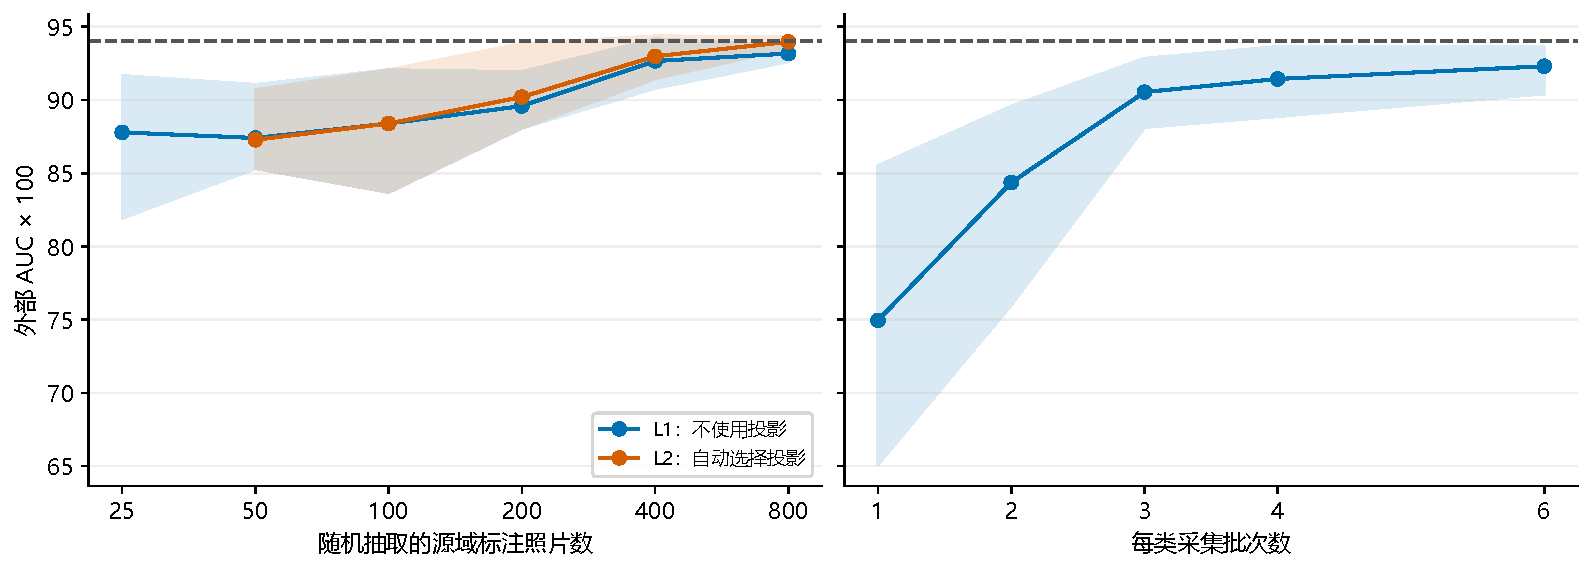
\includegraphics[width=1.0\linewidth,height=.74\textheight,keepaspectratio]{fig17_data_curves.pdf}
\caption{标注数量与采集批次覆盖曲线。随机图像曲线每个条件三次运行，采集批次曲线每个条件五次运行。色带是最小值至最大值。虚线为全量 1,934 张源域训练的 L1。各曲线采用表~\ref{tab:coverage} 所列的独立抽样配置。}
\label{fig:curves}
\end{figure}

\subsection{学生训练设置与随机重复}
\label{app:student_settings}
参数与数值处理决定同一 STAND 框架的具体运行方式。我们按选样规则、训练轮数、分支标准化和随机种子组织补充对照，每组保留相应主配置与全部已报告设置，结果见表~\ref{tab:student_settings}。这些实验用于评价配置敏感性，正文表~\ref{tab:ablation} 则比较组件和训练策略的改变。

\begin{table}[htbp]
\centering\small
\caption{STAND 的训练设置敏感性与随机重复（\%）。每个实验区均列出主配置作为参照，粗体表示该区各性能列最高值，显示精度下并列最高均加粗。分支统计的定义见表~\ref{tab:normalization}。随机种子仅改变学生局部头的训练抽样。开发集用于配置选择，开发期间的测试查看情况见第~\ref{sec:comparison} 节。}
\label{tab:student_settings}
\begin{adjustbox}{max width=\linewidth}
\begin{tabular}{lrrrrrr}
\toprule
配置 & 伪标签数 & 开发 AUC & 开发准确率 & 测试 AUC & 测试准确率 & \makecell{测试调整\\阈值准确率}\\
\midrule
\multicolumn{7}{l}{\textit{伪标签选样设置}}\\
STAND（组成配额 $\rho=0.6$） & 1785 & \textbf{97.85} & \textbf{93.74} & \textbf{97.25} & \textbf{91.38} & 91.06\\
组成配额 $\rho=0.4$ & 1190 & 96.99 & 92.03 & 96.39 & 89.22 & 88.85\\
组成配额 $\rho=0.8$ & 2380 & 97.81 & 93.17 & 97.15 & 91.27 & \textbf{91.76}\\
固定两端各 20\% & 1190 & 96.52 & 91.27 & 95.87 & 87.93 & 87.45\\
固定两端各 30\% & 1784 & 97.69 & 93.55 & 97.07 & 90.57 & 90.95\\
固定两端各 40\% & 2380 & 97.61 & 92.60 & 97.00 & 91.11 & 91.22\\
混合后验 $\geq0.8$ & 2594 & 97.02 & 89.37 & 96.24 & 87.45 & 88.79\\
混合后验 $\geq0.9$ & 2279 & 97.01 & 88.24 & 96.27 & 86.26 & 88.04\\
\midrule
\multicolumn{7}{l}{\textit{自训练轮数}}\\
一轮自训练 & 1785 & 97.35 & 92.03 & 96.79 & 91.06 & 90.73\\
STAND（两轮自训练） & 1785 & \textbf{97.85} & \textbf{93.74} & \textbf{97.25} & \textbf{91.38} & \textbf{91.06}\\
三轮自训练 & 1785 & 97.81 & \textbf{93.74} & 97.20 & 91.16 & 90.95\\
\midrule
\multicolumn{7}{l}{\textit{分支标准化统计}}\\
STAND（主配置统计处理） & 1785 & 97.85 & 93.74 & 97.25 & 91.38 & 91.06\\
\makecell[l]{全局用源域统计\\局部用选样统计} & 1785 & \textbf{97.87} & \textbf{93.93} & \textbf{97.31} & \textbf{91.54} & \textbf{91.38}\\
\midrule
\multicolumn{7}{l}{\textit{随机种子}}\\
STAND（种子 0） & 1785 & \textbf{97.85} & \textbf{93.74} & \textbf{97.25} & \textbf{91.38} & 91.06\\
STAND（种子 1） & 1785 & 97.77 & 93.55 & 97.20 & 91.22 & \textbf{91.27}\\
STAND（种子 2） & 1785 & 97.79 & \textbf{93.74} & 97.18 & 91.11 & 90.95\\
\bottomrule
\end{tabular}
\end{adjustbox}
\end{table}


两轮训练保持正负伪标签配额不变，并利用第一轮学生重新选择照片。其 AUC 与默认准确率均高于一轮设置。增加到三轮后，结果与两轮接近。不同选样比例同时改变训练规模和入选照片的可靠性，$\rho=0.8$ 的调整阈值准确率高于主配置，而主配置在这一选样组的默认准确率和 AUC 最高。这表明参数对排序和阈值决策可能产生不同影响，应结合实际采用的输出规则评价。

标准化对照采用“全局用源域统计、局部用选样统计”。具体而言，全局分类头在训练和评分时均使用源域特征均值与标准差，局部分类头则始终保留当前伪标签子集的图像块统计量，不在评分前替换为完整目标池统计量。主配置的对应处理见表~\ref{tab:normalization}。该对照同时改变两个分支，在本次运行中的开发 AUC、开发准确率、测试 AUC 和默认测试准确率均略高于主配置。结果支持标准化方式会影响分类器的具体表现，当前证据不将主配置解释为标准化选择中的最优设置。

三个种子的测试 AUC 为 97.18--97.25，默认准确率为 91.11\%--91.38\%，说明当前主配置在这些重复运行中表现接近。标准化对照仅有一次运行，不能将其小幅领先直接解释为稳定的泛化增益。开发与测试 AUC 的完整设置对照见图~\ref{fig:distill}，其中同时保留正文的组件变体与本节的参数配置，以便核查各项变化。

\begin{figure}[htbp]
\centering
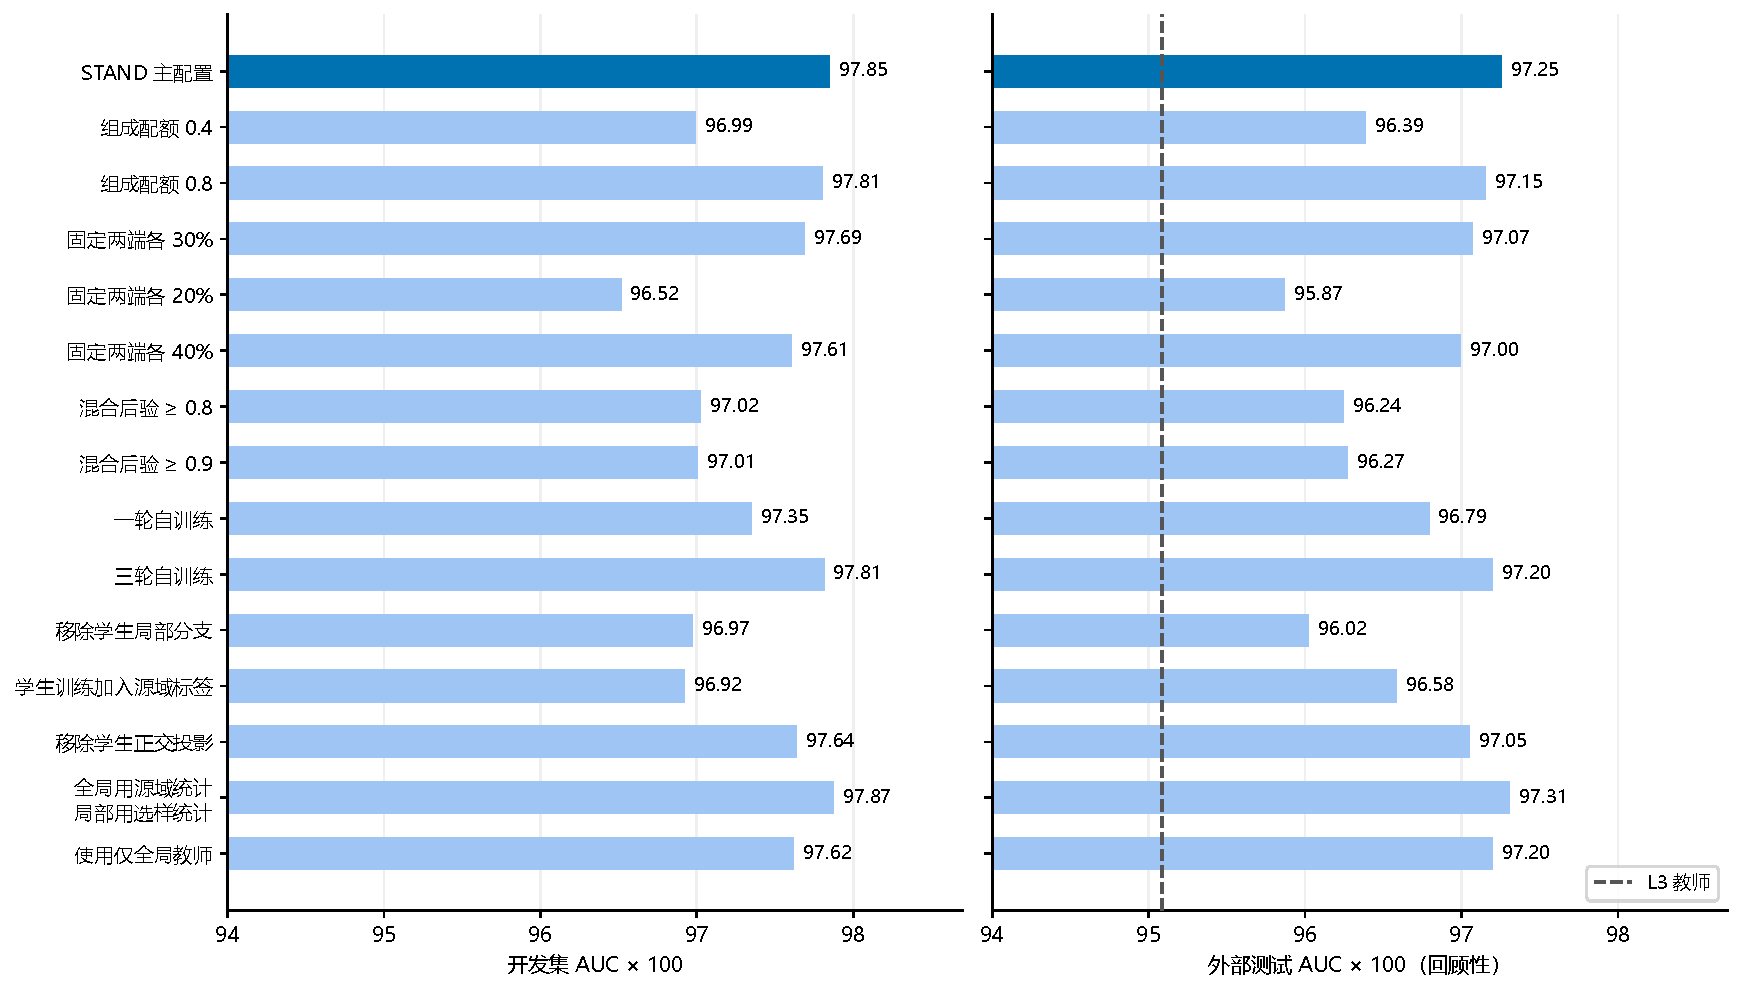
\includegraphics[width=1.0\linewidth,height=.74\textheight,keepaspectratio]{fig15_distillation_choices.pdf}
\caption{STAND 组件与训练设置的开发及外部测试 AUC。虚线为未适应 L3 教师。标准化变体的“全局用源域统计、局部用选样统计”含义见正文及表~\ref{tab:normalization}。本图保留全部原有配置，开发与测试数据的使用情况见第~\ref{sec:comparison} 节。}
\label{fig:distill}
\end{figure}

\subsection{训练数据与标准化的对应关系}
固定编码器并不等于训练过程中所有数值变换都固定。标准化改变特征各维的中心与尺度，分类权重则决定这些坐标如何形成分数，因此需要同时明确两者的训练数据。各分支的对应关系列于表~\ref{tab:normalization}。主配置的局部学生在伪标签子集统计下训练，在完整池统计下评分，使性能同时受到样本选择、分类权重和标准化处理的影响。学生对照所检验的是这些更新的整体效果，因此，各种统计处理应结合分类头拟合方式分析。

实现中，全局头使用逐维总体标准差，局部头采用当前张量实现的标准差计算，并分别加入 $10^{-8}$ 和 $10^{-6}$。源域投影基在学生阶段保持固定，主配置使用的目标统计量仅取自独立适应池 $\mathcal U$。补充标准化对照将全局头改为源域统计、局部头保留伪标签子集统计，两处分支更新共同对应表~\ref{tab:student_settings} 中的标准化实验。

\begin{table}[htbp]
\centering\small
\caption{教师、STAND 主配置与标准化变体的拟合样本及统计量。$\mathcal Q_r$ 为第 $r$ 轮伪标签子集。末两行为“全局用源域统计、局部用选样统计”配置。}
\label{tab:normalization}
\begin{adjustbox}{max width=\linewidth}
\begin{tabular}{llll}
\toprule
分支 & 拟合样本 & 训练时统计量 & 评分时统计量\\
\midrule
教师全局头 & $\mathcal S$ & 源域全局特征 & 源域全局特征\\
教师局部头 & $\mathcal S$ & 源域所有图像块 & 源域所有图像块\\
学生全局头（主配置） & $\mathcal Q_r$ & 完整 $\mathcal U$ 全局特征 & 完整 $\mathcal U$ 全局特征\\
学生局部头（主配置） & $\mathcal Q_r$ & $\mathcal Q_r$ 所有图像块 & 完整 $\mathcal U$ 所有图像块\\
\midrule
学生全局头（变体） & $\mathcal Q_r$ & 源域全局特征 & 源域全局特征\\
学生局部头（变体） & $\mathcal Q_r$ & $\mathcal Q_r$ 所有图像块 & $\mathcal Q_r$ 所有图像块\\
\bottomrule
\end{tabular}
\end{adjustbox}
\end{table}

训练实现采用统一且明确的增强和优化配置。CNN 的裁剪面积比例为 0.6--1.0。几何增强包括随机水平翻转、$\pm15^\circ$ 仿射旋转和最多 10\% 的平移。随机灰度化的概率为 0.1，亮度、对比度和饱和度扰动的幅度均为 0.2。AdamW 权重衰减为 $10^{-2}$，梯度范数截断为 1.0，学习率保持固定。EfficientNetV2-S、Inception-v3、MobileNetV3-Large 和 ResNet-50 的输入边长分别为 384、299、224 和 224。DINOv3 与 SigLIP~2 权重标识分别为 \path{vit_base_patch16_dinov3.lvd1689m} 和 \path{google/siglip2-base-patch16-224}。这些配置将基线训练、冻结表征和内容筛选的条件具体化，为比较结果提供可核查的实现依据。

\subsection{关键结果的统计解释}
统计分析以图像级指标和拍摄者级重采样相结合。准确率、精确率、召回率及 F1 在图像层面计算，聚类 bootstrap 整组抽取拍摄者并保留其全部照片，使同一拍摄者内部的相关性在重采样中得到保留。四种微调 CNN 用三个种子的指标均值描述训练重复，单模型区间描述固定模型的拍摄者采样变化，照片池敏感性范围描述两次运行的最小值和最大值。明确区分这些统计对象，使主性能、随机重复与组成敏感性的证据各自对应所评价的问题。


\subsection{公众照片来源与许可}
定性案例的解释需要能够回到原始照片核查。公众照片的模型预测、可见外观和平台弱标签并不完全等同，观察记录能够帮助检查它们之间的关系。本文保留成功与困难案例的原始观察编号和许可，并在表~\ref{tab:credits} 中列出对应来源。采用相同的核查方式，可以避免只对纠正案例作有利解释，也便于结合原图判断局部响应的含义。该表用于保证案例分析可追溯。

\begin{table}[htbp]
\centering\small
\caption{局部响应与失败案例的原始公众照片记录及许可。观察编号可点击跳转。图中照片曾缩放并叠加响应图。部分素材为 CC BY-NC，应遵守原许可。数据示例图的公众照片为 CC0 或 CC BY，源域照片许可见原始数据存档。该表为来源说明，不适用指标加粗规则。}
\label{tab:credits}
\begin{adjustbox}{max width=\linewidth}
\begin{tabular}{lrr}
\toprule
案例角色 & iNaturalist 观察编号 & 许可\\
\midrule
公开模型漏检、学生检出 & \href{https://inaturalist.org/observations/166493572}{166493572} & cc-by-nc\\
公开模型漏检、学生检出 & \href{https://inaturalist.org/observations/165836329}{165836329} & cc-by-nc\\
公开模型漏检、学生检出 & \href{https://inaturalist.org/observations/14213937}{14213937} & cc-by-nc\\
公开模型漏检、学生检出 & \href{https://inaturalist.org/observations/121473483}{121473483} & cc-by-nc\\
两者均检出 & \href{https://inaturalist.org/observations/217885053}{217885053} & cc0\\
两者均检出 & \href{https://inaturalist.org/observations/180065254}{180065254} & cc-by\\
学生正确判为负类 & \href{https://inaturalist.org/observations/212769317}{212769317} & cc-by-nc\\
学生正确判为负类 & \href{https://inaturalist.org/observations/115204794}{115204794} & cc-by-nc\\
学生正确判为负类 & \href{https://inaturalist.org/observations/76417846}{76417846} & cc-by-nc\\
学生漏检 & \href{https://inaturalist.org/observations/165825387}{165825387} & cc-by\\
学生漏检 & \href{https://inaturalist.org/observations/290504159}{290504159} & cc-by-nc\\
学生误报 & \href{https://inaturalist.org/observations/405042952}{405042952} & cc-by-nc\\
学生误报 & \href{https://inaturalist.org/observations/162166322}{162166322} & cc-by-nc\\
\bottomrule
\end{tabular}
\end{adjustbox}
\end{table}


\FloatBarrier
\end{document}
